\chapter{A Continuous Stored Energy Vertex Model with Nucleation}
\label{chap:storedenergy}

\lettrine{E}{xtensions} of the classic Vertex Model \cite{torres2015} considers the introduction of an intragranular stored energy $\SE$ which plays a key role in primary recrystallization, that is, the generation of new grains before the grain growth regime~\cite{pikekos2008generalized, pikekos2008stochastic}.
This process will significantly modify the material and produce drastic changes of many physical properties like electrical resistance, internal stresses, micro-hardness, among others, see~\cite{pikekos2008generalized, pikekos2008stochastic}.
Vertex Model implementations defining the structure as a graph, as presented in Chapter~\ref{chap:2dgrains}, are common but models that include nucleation are rare since the data structure does not allow dislocation inside grains~\cite{Orend2015}.

In this chapter, we first introduce the evolution equations of vertices considering the stored energy term and then we analyze the nucleation process.

Following the notation from~\cite{pikekos2008stochastic}, 
the local energy of a vertex $i$ considering the stored energy term is defined as:
 \begin{equation*}
     E_i = \sum_{j \in \mathcal{N}_i}\left(\gamma^{(i,j)}\AL_{i,j} + \SE_{i,j}A_{i,j}\right),
 \end{equation*}
 %
 where $\mathcal{N}_i$ is the set of neighbor vertices to the vertex $i$, $\gamma^{(i,j)}$ and $\AL_{i,j}$ are the grain boundary energy and the arc length of the boundary formed by vertices $i$ and $j$, $\SE_{i,j}$ and $A_{i,j}$ is the stored energy and area of a grain adjacent to the boundary $i,j$ using the right-hand rule.  We split the local energy between the grain boundary contribution and the grain area contribution, so:
 \begin{equation*}
     E_i = \sum_{j=1}^3 \gamma^{(k_{i,j})}\AL_{k_{i,j}} + \sum_{j=1}^3 \SE_{g_{i,j}}A_{g_{i,j}},
 \end{equation*}
 %
 where $k_{i,\cdot}$ and $g_{i,\cdot}$ are indices for the three boundaries and grains relative to vertex~$i$. Now, we could define the total energy of the system as:
 %where $\boundaries_i$ and $\grains_i$ are the sets of boundaries and grains associated to vertex $i$ respectively. Now, we could define the total energy of the system as:
 \begin{equation}
     E = \sum_{k = 1}^{K} \gamma^{(k)}\AL_{k} + 
     \sum_{g = 1}^{N} \SE_{g}A_{g}.
     \label{eq:SEtotalenergy}
 \end{equation}
%
 where $K$ and $N$ are total number of boundaries and grains respectively. So, now we could decompose the contribution from each vertex to the total energy as follows,
 \begin{equation}
     \widehat{E}_i = \sum_{j=1}^3 \gamma^{(k_{i,j})}\dfrac{\AL_{k_{i,j}}}{2} + \sum_{j=1}^3 \SE_{g_{i,j}}\dfrac{A_{g_{i,j}}}{\ns(g_{i,j})},
        \label{eq:SEvertexenergy}
 \end{equation}
 %
 where $\ns(g)$ is the number of sides (or class) of grain $g$. This allows us to build the total energy
 as the sum of the contribution of each vertex such that we ensure we only consider once each grain boundary contribution and also consider once each grain contribution, thus,
 \begin{align*}
     \sum_{i=1}^{M} \widehat{E}_i %&= \sum_{k=1}^{K} \gamma^{(k)} \frac{\AL_k}{2} + \sum_{g=1}^{N} \SE_{g}\frac{A_g}{\ns(g)} \\
      &= \underbrace{\sum_{i = 1}^{M} \sum_{j=1}^3 \gamma^{(k_{i,j})} \frac{\AL_{k_{i,j}}}{2} }_{(a)}
     + \underbrace{\sum_{i = 1}^{M} \sum_{j=1}^3 \SE_{g_{i,j}} \frac{A_{g_{i,j}}}{\ns(g_{i,j})} }_{(b)}
 \end{align*}
 In order to compute $(a)$ we need to understand which elements are being counted. Consider an specific vertex $i$ and their related boundaries. The expansion of $(a)$ for vertex $i$ looks like:
\begin{equation*}
    \gamma^{(k_{i,1})}\frac{\AL_{k_{i,1}}}{2} + \gamma^{(k_{i,2})}\frac{\AL_{k_{i,2}}}{2} + \gamma^{(k_{i,3})}\frac{\AL_{k_{i,3}}}{2}.
\end{equation*}
The same term for some neighbor vertex looks like:
\begin{equation*}
    \gamma^{(k_{1,i})}\frac{\AL_{k_{1,i}}}{2} +
    \gamma^{(k_{1,\cdot})}\frac{\AL_{k_{1,\cdot}}}{2} +
    \gamma^{(k_{1,\cdot})}\frac{\AL_{k_{1,\cdot}}}{2}.
\end{equation*}
%
It is clear that for each vertex we are counting the grain boundary energy and arc length twice, each time per vertex in a boundary. 
This justifies the introduction of the term $1/2$ in $(a)$. The analysis for $(b)$ holds a similar argument. 
The inner sum of here runs over the grains related to vertex $i$.  We can build a similar example starting from a vertex $i$ and counting the three stored energy terms related as:
\begin{equation*}
    \SE_{g_{i,1}}\frac{A_{g_{i,1}}}{\ns(g_{i,1})} + \SE_{g_{i,2}}\frac{A_{g_{i,2}}}{\ns(g_{i,2})} +
    \SE_{g_{i,3}}\frac{A_{g_{i,3}}}{\ns(g_{i,3})}.
\end{equation*}
Consider now that grain $g_{i,1}$ has $\ns(g_{i,1})$. We already know that vertex $i$ forms part of that grain. The other $\ns(g_{i,1})-1$ vertices of $g_{i,1}$ have also in their stored energy terms the term $\SE_{g_{i,1}}\dfrac{A_{g_{i,1}}}{\ns(g_{i,1})}$ and thus we are adding the same term $\ns(g_{i,1})$ times. This justifies the introduction of the term $1/\ns(g)$. Finally we can map the sum in order to count boundaries and grains. 
Each term related to a boundary is counted twice and each term related to a grain is counted $\ns(g)$ times and we can recover an expression for the total energy of the system as:
\begin{align*}
    \sum_{i=1}^{M} \widehat{E}_i &= \sum_{k=1}^{K} 2 \cdot \gamma^{(k)} \frac{\AL_{k}}{2} + \sum_{g=1}^{N} \ns(g)\cdot\SE_{g}\frac{A_g}{\ns(g)}\\
    &= \sum_{k=1}^{K} \gamma^{(k)} \AL_{k} + \sum_{g=1}^{N} \SE_{g} A_g\\
    &= E.
\end{align*}
If we explicit the dependency of the boundary arc lengths and grain areas with respect to the vertices positions $\{\x_i=\langle x_i,y_i\rangle\}$ we can build the evolution equations for this model such that it decreases its energy by a gradient descent method, that is to compute $\dotx_{i}(t) = \left\langle -\dfrac{\partial E}{\partial x_i}, -\dfrac{\partial E}{\partial y_i}\right\rangle$.

\section{Numerical Algorithm}
\label{sec:se_numerical}

Computing the \emph{velocity} of each vertex is actually the computation of the gradient of the energy $E$ from equation \eqref{eq:SEtotalenergy}.
Here we propose a matrix-free approach to approximate the gradient.
The main advantage of this approach is that it only needs 
the implementation of computation of the total energy of the system, 
this greatly simplifies the bookkeeping we would need to handle this task.

A convenient way to approximate each partial derivative is with a  matrix-free approach.
Consider the vector $\X \in \mathbb{R}^{2M}$ of stacked components of 
$\x_i$, this is:
\begin{equation*}
    \X = (x_1, x_2, \cdots, x_M, y_1, y_2, \cdots, y_M)^T,
\end{equation*}
where $M$ is the total number of triple junctions and $^T$ is the transpose operator.
Each $m$-th component of the gradient for this vector, 
say $\dfrac{\partial E(\X)}{\partial \X_m}$ is approximated by:
%
\begin{equation}
    \frac{\partial E(\X)}{\partial \X_m} \approx 
    \frac{E(\X + \varepsilon\,  \ei{m}) - E(\X)}{\varepsilon},
    \label{eq:partialE}
\end{equation}
%
where $\ei{m}$ is the $m$-th canonical vector in $\mathbb{R}^{2M}$. The numerical evaluation of this approximation implies that the energy of the system must be recomputed twice for each vertex, 
one to compute $E(\X)$ and the second one is $E(\X + \varepsilon\,  \ei{m})$, where a small perturbation is added to the $m$-th component. According to \eqref{eq:SEtotalenergy}, this means to recompute each individual vertex energy each time.
Fortunately, this can be handled efficiently by pointing out 
which terms will be changed after the perturbation.

A quadratic cost would be required for a naive implementation.
A more detailed analysis shows that the perturbation only affects the $x$ or $y$ component of a vertex $\x_i$, which implies that only the three related grain areas and the three grain boundary arc lengths connected to vertex $\x_i$ will change, as shown in Figure~\ref{fig:delta_energy}.
%
\begin{figure}[t]
    \centering
    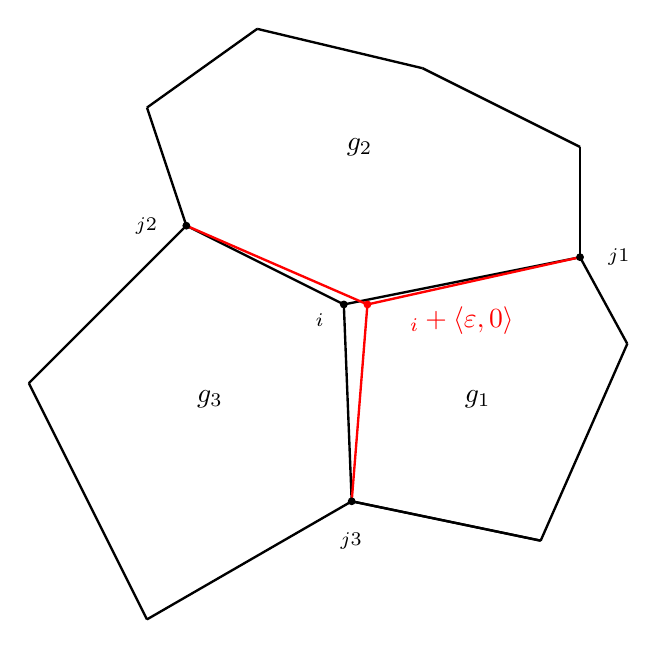
\begin{tikzpicture}
        % boundaries
        % grain 1
        \draw[line width=0.3mm, black] (0,0) -- (3,0.6);
        \draw[line width=0.3mm, black] (3,0.6) -- (3.6,-0.5);
        \draw[line width=0.3mm, black] (3.6,-0.5) -- (2.5, -3);
        \draw[line width=0.3mm, black] (2.5,-3) -- (0.1, -2.5);
        \draw[line width=0.3mm, black] (0.1,-2.5) -- (0,0);
        % grain 2
        \draw[line width=0.3mm, black] (2.5,-3) -- (0.1, -2.5);
        \draw[line width=0.3mm, black] (0,0) -- (-2, 1);
        \draw[line width=0.3mm, black] (-2,1) -- (-4, -1);
        \draw[line width=0.3mm, black] (-4,-1) -- (-2.5, -4);
        \draw[line width=0.3mm, black] (-2.5,-4) -- (0.1, -2.5);
        % grain 3
        \draw[line width=0.3mm, black] (-2,1) -- (-2.5, 2.5);
        \draw[line width=0.3mm, black] (-2.5,2.5) -- (-1.1, 3.5);
        \draw[line width=0.3mm, black] (-1.1,3.5) -- (1,3);
        \draw[line width=0.3mm, black] (1,3) -- (3,2);
        \draw[line width=0.3mm, black] (3,2) -- (3,0.6);
        % Perturbed data
        \draw[line width=0.3mm, red] (0.3,0) -- (3,0.6);
        \draw[line width=0.3mm, red] (0.3,0) -- (-2,1);
        \draw[line width=0.3mm, red] (0.3,0) -- (0.1,-2.5);
        % vertices
        \filldraw [black] (0,0) circle (1.2pt);
        \filldraw [black] (3,0.6) circle (1.2pt);
        \filldraw [black] (-2,1) circle (1.2pt);
        \filldraw [black] (0.1,-2.5) circle (1.2pt);
        \filldraw [red] (0.3,0) circle (1.2pt);
        \node[draw=none, color=black] at (-0.3, -0.2) {$\x_i$};
        \node[draw=none, color=red] at (1.5, -0.2) {$\x_i + \langle \varepsilon,0 \rangle$};
        \node[draw=none, color=black] at (3.5, 0.6) {$\x_{j1}$};
        \node[draw=none, color=black] at (-2.5, 1) {$\x_{j2}$};
        \node[draw=none, color=black] at (0.1, -3) {$\x_{j3}$};
        \node[draw=none, color=black] at (0.2, 2) {$g_2$};
        \node[draw=none, color=black] at (-1.7, -1.2) {$g_3$};
        \node[draw=none, color=black] at (1.7, -1.2) {$g_1$};
    \end{tikzpicture}
    \caption[Vertex perturbation in Stored Energy model]{Sketch of  modified component related to vertex $\x_i$, \ie neighboring arc lengths and areas get modified.}
    \label{fig:delta_energy}
\end{figure}
So, instead of recomputing the energy for each one of the $2M$ components of the gradient, we can compute directly the
difference of energies given by the perturbation.
Expanding the difference of energies from \eqref{eq:partialE} and taking into account that the perturbation effect is local, we obtain:
\begin{align*}
    E(\X+\varepsilon\,  \ei{m}) - E(\X) &=  
    \sum_{k =1}^K \gamma^{(k)}\Delta{\AL}_{k} + 
     \sum_{g=1}^N \SE_{g}\Delta{A}_{g}\\
    &= \sum_{j=1}^3 \gamma^{(k_{i,j})} \Delta \AL_{k_{i,j}} + \sum_{j=1}^3 \SE_{g_{i,j}} \Delta A_{g_{i,j}},
\end{align*}
where $i=m \bmod M$.  Notice that the three boundaries and grain areas are modified by adding a perturbation to the vertex $i$. Now, dividing by $\varepsilon$ we obtain the right-hand-side of \eqref{eq:partialE}, \begin{align*}
    \dfrac{E(\X+\varepsilon\,  \ei{k}) - E(\X)}{\varepsilon} &=  
    \sum_{j =1}^3 \gamma^{(k_{i,j})} \dfrac{\Delta{\AL}_{k_{i,j}}}{\varepsilon}
     +\sum_{j=1}^3 \SE_{g_{i,j}}\dfrac{\Delta{A}_{g_{i,j}}}{\varepsilon}
\end{align*}
%
Moreover, each estimation of the gradient can be computed efficiently in parallel since only local information of areas and arc lengths is needed.

\section{The Stored Energy Effect Over the Dynamics of a Triple Junction}
\label{sec:dynamics} 
 
This section studies how the stored energy %values
affects the configuration and stability of the grain network.
We extend the stability study in~\cite{Bernacki2011} where they only analyze stable configurations.

Considering a bounded domain where three grains coexists,
where two of them have the same stored energy, \ie $\SE_1=\SE_2$, and
the third has a different stored energy $\SE_3$ as 
shown in Figure~\ref{fig:segrains}.
%
\begin{figure}
    \centering
    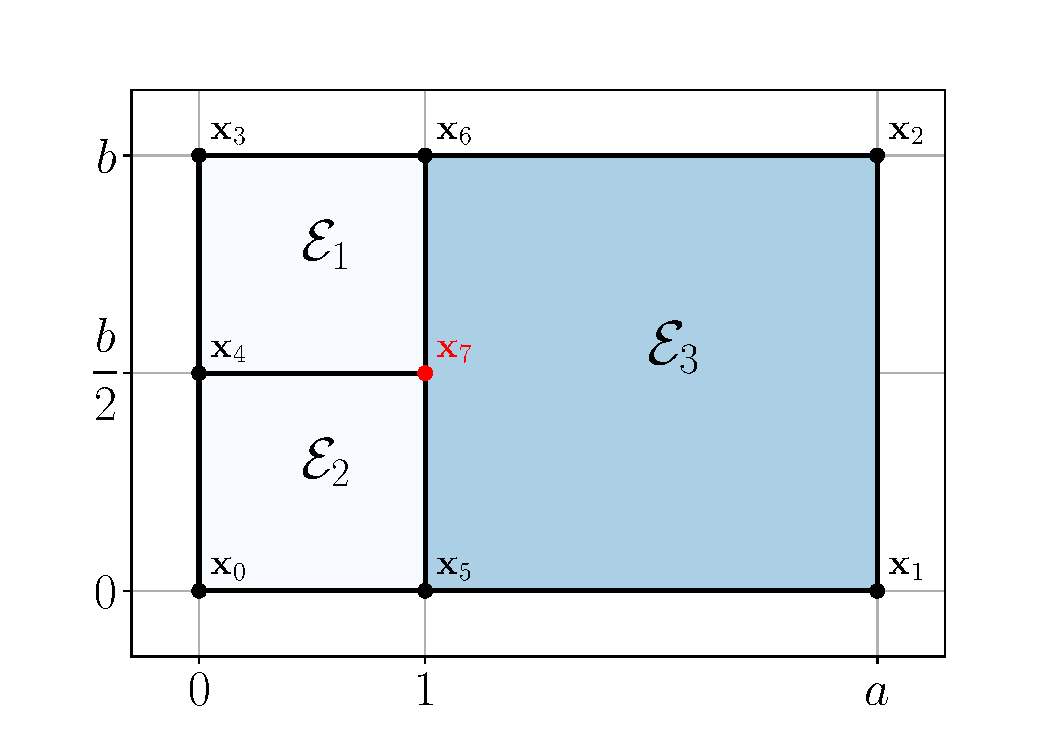
\includegraphics[scale=0.5]{figures/stored_energy/SE_analysis.pdf}
    \caption[Configuration of three grains with different values of stored energy and a vertex with one degree of freedom]{Configuration of three grains with different values of stored energy and a vertex with one degree of freedom (red dot). Initially the dot is placed at $(1,\frac{b}{2})$.}
    \label{fig:segrains}
\end{figure}
%
To measure the effect of the stored energy we let the central vertex located at $(x, b/2)$ 
to freely move, due to symmetry this only happens along the $x$-axis. 
Let $A_1$, $A_2$, $A_3$ the areas of the grains with stored energy $\SE_1$, $\SE_2$ and $\SE_3$, respectively.  Grain areas can be explicitly computed as:
%
\begin{align}
    A_1 &= A_2 = \frac{b\,(1+x)}{4}, & A_3 = a\,b - \frac{b\,(1+x)}{2}.
    \label{eq:SEareas}
\end{align}
%
We now compute each local stored energy based on~\ref{eq:SEvertexenergy}.
Grain class for $A_1$ and $A_2$ is four and for $A_3$ is five. 
Notice that in this domain, boundaries on the edges are not 
counted twice per grain, thus they are not divided by 2.
We also assume %$\SE_1=\SE_2$ and
$\SE_3>\SE_1$.
%
\begin{align*}
\widehat{E}_0 &= \widehat{E}_3 = 1+\frac{b}{2} + \SE_1\,\frac{b\,(1+x)}{16}\\
\widehat{E}_1 &= \widehat{E}_2 = a - 1 + b + \SE_3 \frac{a b - \frac{b (1 + x)}{2}}{5}\\
\widehat{E}_4 &= b + \frac{x}{2} + \SE_1\frac{A_1}{2}\\
\widehat{E}_5 &= \widehat{E}_6 = a + \frac{\sqrt{(x-1)^2 + (b/2)^2}}{2} + \SE_1\frac{b(1+x)}{16} + \SE_3\frac{ab - \frac{b (1 + x)}{2}}{5}\\
\widehat{E}_6 &= \frac{x}{2} + \sqrt{(x-1)^2 + (b/2)^2} + \SE_1\frac{b (1 + x)}{8} + \SE_3 \frac{a b - \frac{b (1 + x)}{2} }{5}
\end{align*}
%
If we add up all the individual energy terms and replace the definitions of areas in \eqref{eq:SEareas}, the total energy becomes:
\begin{equation}
    E = \sqrt{b^2 + 4\,(-1 + x)^2} + x + a\, (4 + b\,\SE_3) + 
 \frac{b\,(8 + \SE_1\,(x+1) - \SE_3\,(1 + x))}{2}.
    \label{eq:SEtotalenergyexample}
\end{equation}
If we compute the derivative of \eqref{eq:SEtotalenergyexample} with respect to $x$ we obtain
\begin{equation}
    \frac{dE}{dx} = 1 + \frac{4 (x-1)}{\sqrt{b^2 + 4 (x-1)^2}} - \frac{b \Delta \SE}{2}
    \label{eq:deltaSE}
\end{equation}
%
where $\Delta \SE = \SE_3 - \SE_1$. 
Thus, the motion of the central vertex is influenced by the difference of stored energies and the height of the domain $b$. 
The domain width $a$ does not affect the steady state. 
The steady state can be found making \eqref{eq:deltaSE} equal to 0, which yields the following roots:
\begin{equation}
    x=\frac{ -24 + 2\, b\, \Delta \SE  (b \,\Delta \SE -4) \pm \sqrt{-b^2 \,(b \Delta \SE -6)\, (b \,\Delta \SE -2)^2\, (b\, \Delta \SE +2)}}{2 \,(b\, \Delta \SE -6) (b\, \Delta \SE +2)}.
    \label{eq:xpos_steady}
\end{equation}
When $\Delta \SE = 0$, the domain height $b$ conditions the position of the steady state which is at:
\begin{equation*}
    x_{\text{steady}} = x_+ = 1 - \frac{b}{2\sqrt{3}}.
\end{equation*}
%By analyzing the obtained roots only one solution will have physical sense. 
By analyzing the obtained roots only $x_+$ has physical sense.
The critical point, assuming $\Delta \SE > 0$, is just before 
the squared root in \eqref{eq:xpos_steady} becomes complex. 
This is at $b\Delta \SE = 6$ and solutions with $b \Delta \SE < 6$ will be real and will be a valid steady states, as shown in Figure~\ref{fig:SE_stability}. 
From the numerical point of view several experiments were performed by estimating $\dfrac{dE}{dx}$ with the matrix-free approach. 
As this approach will not capture complex solutions, from $b\Delta \SE \geq 6$ the solutions become unstable and unbounded, as shown in Figure~\ref{fig:SE_experiments}.

\begin{figure}[t]
    \centering
    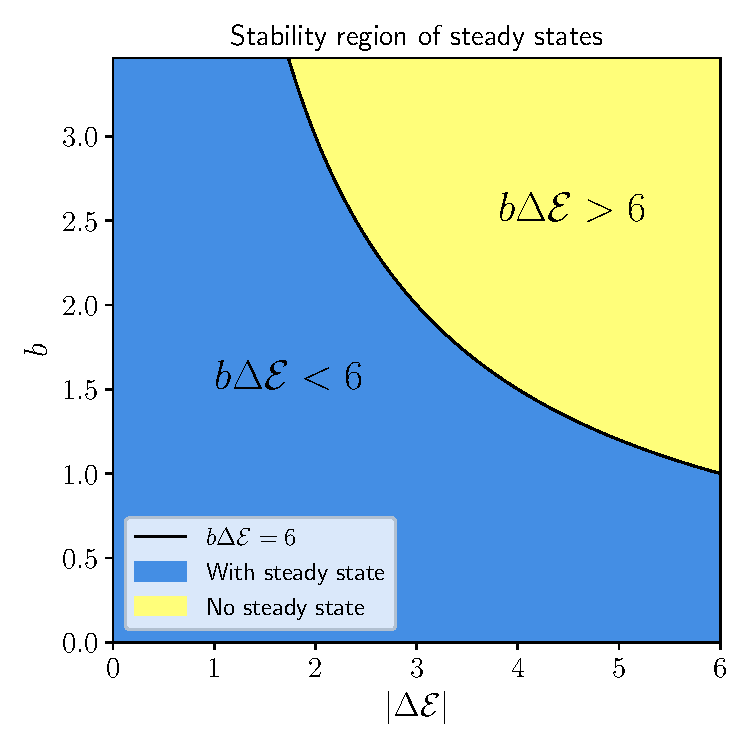
\includegraphics[scale=0.6]{figures/stored_energy/SE_stability.pdf}
    \caption{Stability regions for the relation of $b$ and $\Delta \SE$ in the three grains experiment.}
    \label{fig:SE_stability}
\end{figure}

The concept of stability here refers to the interpretation of the vertex location in the domain.
If the vertex stays inside the three grains we say that it is an steady state.
If the vertex penetrates a grain without stopping, the configuration is said to be unstable.
%since there is no physical meaning for that configuration. 

Figures~\ref{fig:SE_stability_SE0} and~\ref{fig:SE_stability_SE15} shows two valid steady states. Figure~\ref{fig:SE_stability_SE0} shows the steady state when there is no stored energy, therefore the steady state is reached at dihedral angle $2\pi/3$. 
In presence of a large stored energy, the steady state is situated away from the isotropic steady state as shown in Figure~\ref{fig:SE_stability_SE15}. 
Again, when $b\Delta \SE \geq 6$ the solution becomes unbounded.

\begin{figure}
    %\centering
    \hspace{-1em}
    \subfloat[$\SE_1 = \SE_3$.]{
        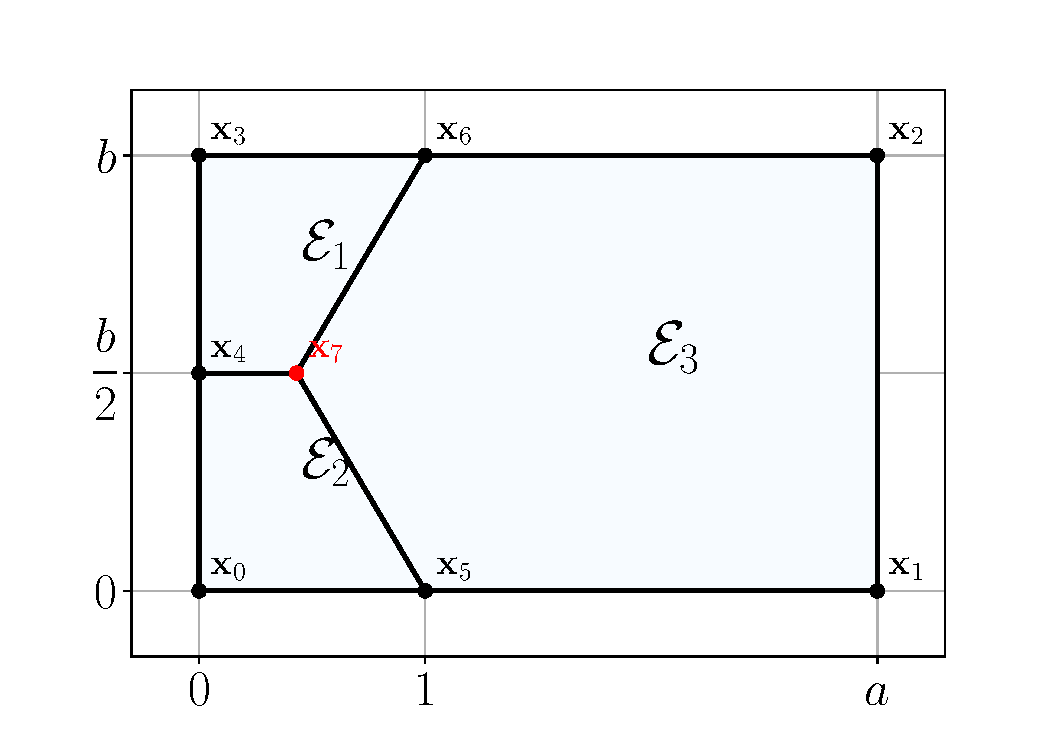
\includegraphics[scale=0.48, trim={2em 0 2em  0}]{figures/stored_energy/SE_analysis_SE0.pdf}
        \label{fig:SE_stability_SE0}
    }
    \subfloat[$\SE_1 < \SE_3$]{
        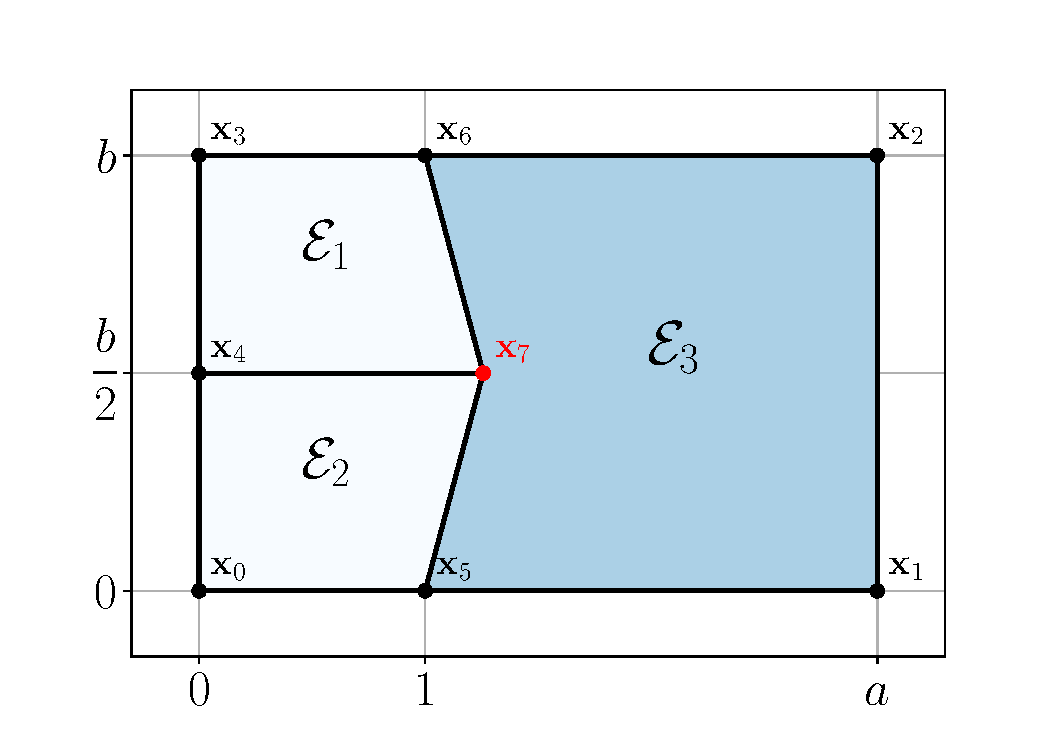
\includegraphics[scale=0.48, trim={2em 0 2em 0}]{figures/stored_energy/SE_analysis_SE1dot5.pdf}
        \label{fig:SE_stability_SE15}
    }
    \caption[Steady states for different configurations of stored energies.]{Steady states for different configurations of stored energies. Notice the magnitude of the perturbed steady state in (b).}
\end{figure}

This estimation can be used as an upper bound for numerical simulations of this model, ensuring that no grains will suffer from instabilities. 
The interpretation is that the parameter $b$ of this study can be %somewhat 
compared to boundaries arc lengths. 
% We can take each arc length and the difference of stored energy of the shared boundary and check the distribution of values for the product $\AL \Delta \SE$. 
% We interpret that this distribution must be bounded to ensure stable simulations.

\begin{figure}
    \centering
    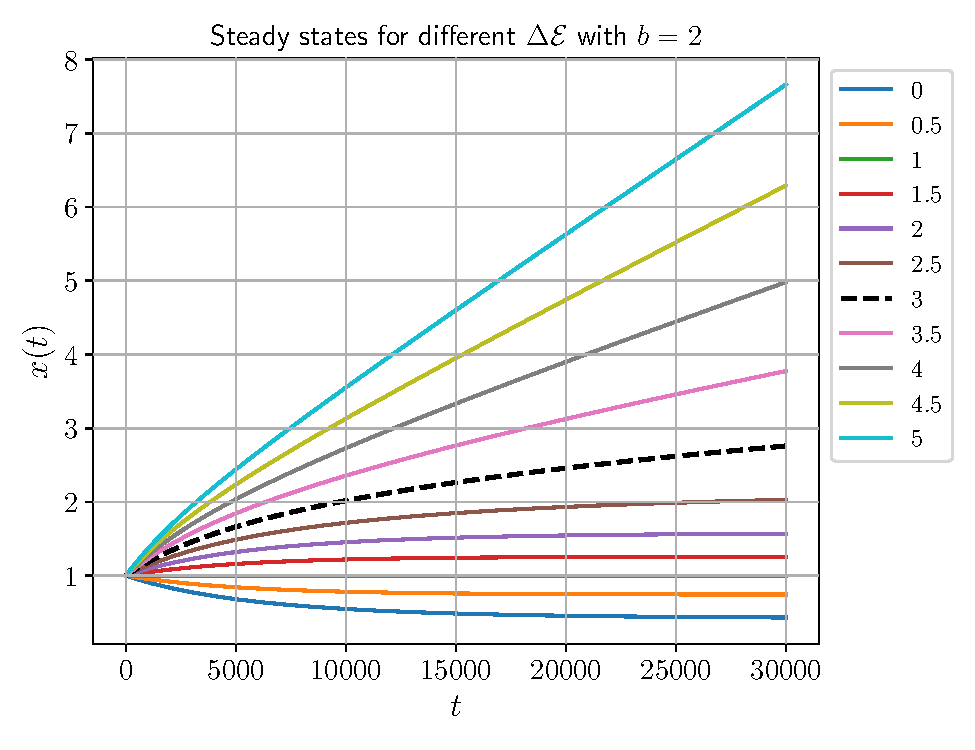
\includegraphics[scale=0.6]{figures/stored_energy/SE_experiments.pdf}
    \caption[Convergence of steady states for a fixed value of $b$ and different values of $b \Delta \SE$]{Convergence of steady states for a fixed value of $b$ and different values of $b \Delta \SE$. Values of $2\,\Delta \SE \geq 6$ become unbounded.}
    \label{fig:SE_experiments}
\end{figure}

\section{The Nucleation Process: Adding a three side Grain and Letting it Grow}
\label{sec:nucleation}

\begin{figure}[t]
    \centering
       \begin{tikzpicture}
        % coordinates
        \coordinate (x1) at (0,-0.5);
        \coordinate (x2) at (0,2.1);
        \coordinate (x3) at (-2,-2.3);
        \coordinate (x4) at (2, -2.3);
        % boundaries
        \draw[line width=0.4mm, red] (x1) -- (x2);
        \draw[line width=0.4mm, red] (x1) -- (x3);
        \draw[line width=0.4mm, red] (x1) -- (x4);
        \draw[line width=0.4mm, black!10!green] (x2) -- (x3);
        \draw[line width=0.4mm, black!10!green] (x3) -- (x4);
        \draw[line width=0.4mm, black!10!green] (x2) -- (x4);
        
        % vertices
        \filldraw [black] (x1) circle (1.5pt);
        \filldraw [black] (x2) circle (1.5pt);
        \filldraw [black] (x3) circle (1.5pt);
        \filldraw [black] (x4) circle (1.5pt);
        
        % Text
        \node[draw=none, color=black, below] at (x1) {$\x_{1}$};
        \node[draw=none, color=black, above] at (x2) {$\x_{2}$};
        \node[draw=none, color=black, below] at (x3) {$\x_{3}$};
        \node[draw=none, color=black, below] at (x4) {$\x_{4}$};
        
        \node[draw=none, color=black, right] at ($(x2)!0.5!(x4)$) {$\AL_{2,4}$};
        \node[draw=none, color=black,left] at ($(x2)!0.5!(x3)$) {$\AL_{2,3}$};
        \node[draw=none, color=black, below] at ($(x3)!0.5!(x4)$) {$\AL_{3,4}$};
        
        \node[draw=none, color=black, right] at ($(x1)!0.35!(x2)$) {$\AL_{1,2}$};
        \node[draw=none, color=black, above] at ($(x1)!0.45!(x3)$) {$\AL_{1,3}$};
        \node[draw=none, color=black, above] at ($(x1)!0.45!(x4)$) {$\AL_{1,4}$};
        
        \node[draw=none, color=black] at ($0.33*(x1)+0.33*(x4)+0.33*(x2)$) {$\color{red}{A_{1}}$};
        \node[draw=none, color=black] at ($0.33*(x1)+0.33*(x2)+0.33*(x3)$) {$\color{red}{A_{2}}$};
        \node[draw=none, color=black] at ($0.33*(x1)+0.33*(x3)+0.33*(x4)$) {$\color{red}{A_{3}}$};
    \end{tikzpicture}
    %\includegraphics[scale=0.4]{figures/nucleation2.pdf}
    \caption{Sketch of energies associated to a 3-side grain before and after it is nucleated. Red shows what it is going to be removed and green what it is going to be added.}
    \label{fig:SE_nucleation2}
\end{figure}

The nucleation process can be classified as a new type of topological change in the system, considering the already well-known topological changes (flipping and  grain removal) described in Chapter~\ref{chap:2dgrains}. 
As usual, this new type of topological change should be energy decreasing, otherwise, it would 
induce the removal of the nucleated grain right away.
To analyze this topological change, we propose the following sketch, see Figure~\ref{fig:SE_nucleation2}.
In this sketch we observe what we call
the current configuration of energy $E_0^{\triangle}$, in red, and a candidate configuration of energy $E_1^{\triangle}$.
The main idea is that for a candidate vertex $\x_1$, where we could perform a nucleation,
we can explicitly compute the difference of energy
before and after the nucleation, i.e. $\Delta E^{\triangle}=E_1^{\triangle}-E_0^{\triangle}$. 
So, as long as the difference is negative we can conclude that nucleation will be successful. 
Thus, the $\Delta E^{\triangle}$ is as follows,
\begin{align}
    E_0^{\triangle} &= \gamma^{(1,2)}\,\AL_{1,2}
    +\gamma^{(1,3)}\,\AL_{1,3}+\gamma^{(1,4)}\,\AL_{1,4}
    +\SE_1\,A_1+\SE_2\,A_2+\SE_3\,A_3,\nonumber\\
    E_1^{\triangle} &= \gamma^{(2,4)}\,\AL_{2,4}
    +\gamma^{(2,3)}\,\AL_{2,3}+\gamma^{(3,4)}\,\AL_{3,4},\nonumber\\
    \Delta E^{\triangle} &= E_1^{\triangle}-E_0^{\triangle},
    \label{eq:Delta_E_Nucleation}
\end{align}
%
where $\x_i$ are the coordinates of the vertex $i$ for $i\in\{1,2,3,4\}$, 
$\AL_{i,j}$ is the arc length from vertex $\x_i$ to vertex $\x_{j}$, $\gamma^{(i,j)}$ is the grain boundary energy from vertex $\x_i$ to vertex $\x_{j}$,  
$A_1$ is the area of grain with vertices $\{\x_1,\x_4,\x_2\}$,
$A_2$ is the area of grain with vertices $\{\x_1,\x_2,\x_3\}$,
$A_3$ is the area of grain with vertices $\{\x_1,\x_3,\x_4\}$,
and $\SE_g$ is the store energy of the grain associated to $A_g$ for $g \in \{1,2,3\}$.


\subsection{A Symmetric Nucleation Analysis}

To gain insight in the general conditions for allowing nucleation, we will consider a particular case.
Specifically, we will consider isotropic grain boundary energy $\gamma$, \ie $\gamma=1$,
$\AL_{1,i}=r$ for $i\in\{2,3,4\}$
$\AL_{2,4}=L$, $\AL_{2,3}=L$, $\AL_{3,4}=L$, and dihedral angle of $2\pi/3$. This leads us to the following simplification
of equation \eqref{eq:Delta_E_Nucleation},
\begin{align*}
    \Delta E^{\triangle} &=
    3\,L-3\,r-
    \underbrace{(\SE_1+\SE_2+\SE_3)}_{\displaystyle{\bar{\SE}}}\,A.
\end{align*}
Moreover, due to symmetry, we have that $L=\sqrt{3}\,r$ and $A=\frac{\sqrt{3}}{4}\,r^2$. 
Thus, we obtain,
\begin{align*}
    \Delta E^{\triangle} &=
    3\,\sqrt{3}\,r-3\,r-
    \bar{\SE}\,\frac{\sqrt{3}}{4}\,r^2\\
    &=3\,r\,\left(\sqrt{3}-1-\frac{\sqrt{3}}{12}\,\bar{\SE}\,r\right).
\end{align*}
From which we found out that there are two critical points
with $\bar{\SE}\neq 0$, these are $r_0=0$ and 
$r_c=\dfrac{4\,(3 - \sqrt{3})}{\bar{\SE}}\approx5.071796\,(\SE_1+\SE_2+\SE_3)^{-1}$.
The first critical point $r_0=0$ indicates that making
a nucleation of area $0$ will add $0$ energy, which
is correct but we are not interested in that case.
On the other hand, the second critical point
is the one we are interested, 
$r_c \approx 5.071796 \,\bar{\SE}^{-1}$,
since from that point on we ensure we are
not increasing the energy of the system and will
let the nucleated grain to grow.
%
\begin{figure}
    \centering
    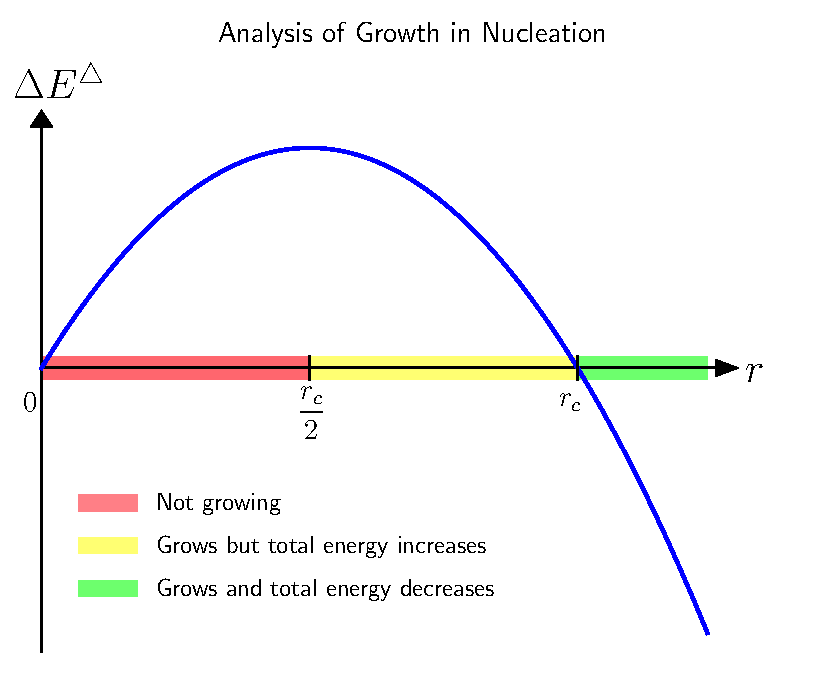
\includegraphics[scale=0.5]{figures/stored_energy/DeltaETriangle.pdf}
    \caption[$\Delta E^{\triangle}$ induced by nucleation in a symmetric case.]{Plot of $\Delta E^{\triangle}$ symmetric with $\bar{\SE}=\SE_1+\SE_2+\SE_3=18$. The ability to growth depends of the size of the nucleated grain.}
    \label{fig:DeltaSE_E6}
\end{figure}
%
In Figure~\ref{fig:DeltaSE_E6} we observe
a qualitative behavior of \eqref{eq:Delta_E_Nucleation} for the symmetric case, this plot shows that we require $r$ from Figure~\ref{fig:SE_nucleation2} to be at least $r_c=4\,(3 - \sqrt{3})\,\bar{\SE}^{-1}$.
This implies to nucleate a large grain,
otherwise we will be adding energy to the system.
An important consideration needs to be made,
if the nucleated grain has radius $r$ in the range
$[0,r_c/2]$, the nucleated grain will not grow.
On the other hand, if the radius of the nucleated grain is 
in the range $]r_c/2,r_c]$,
the nucleated grain will grow but it will initially add
energy to the system,
and when the nucleated grain satisfies $r>r_c$,
the nucleated grain will grown and will
remove energy from the system.
Figure~\ref{fig:DeltaSE_E6} show
these ranges in red, yellow and green, respectively.

\subsection{Analysis of the Nucleated Grain}
For a successful energy decreasing nucleation, 
as discussed in the previous section, 
we have a constraint on the size of the grain to be nucleated.
Otherwise the nucleated grain will not grow. 
Therefore, in the yellow zone there is a potential for a grain to grow but at a cost of a temporal increase of energy. 
The main interest in this type of configuration
is that it imposes a lower requirement for the size
of the grain to make the nucleation successful.

A preliminary analysis indicates %preliminary analysis insight for this to happen is 
that the \emph{slope} of the $\Delta E^{\triangle}$ is negative in that range and an energy decreasing model will favor the enlargement of the grain since it will decrease the energy.
More rigorously, we need to compute $\Delta(\Delta E^{\triangle})=:\Delta^2 E^{\triangle}$.
Figure~\ref{fig:delta2} shows and sketch of two possible nucleation at vertex $\x_1$.
In this case the nucleation on the left is the
one explained previously in Figure~\ref{fig:SE_nucleation2},
which will be denoted as $\Delta E^{\triangle}_1$.
And the one on the right is a nucleation
for a smaller grain for the same vertex $\x_1$,
which will be denoted as $\Delta E^{\triangle}_0$.
These two \emph{virtual} nucleations allow us
to obtain $\Delta^2 E^{\triangle}=\Delta E^{\triangle}_1-\Delta E^{\triangle}_0$.
Thus, if $\Delta^2 E^{\triangle}<0$, we obtain
that the nucleated grain may grow
since it will decrease the energy of the system.
This value will be denoted as the \emph{nucleation
factor}.

Notice that under anisotropic grain boundary energy the computation of $\Delta^2 E^{\triangle}$ will include each grain boundary energy terms, which have to be computed with respect to the orientation of the nucleated grain. By default we set the orientation of the nucleated grain as $\alpha = 0$.


\begin{figure}[t]
    \centering
    \subfloat[$\Delta E^{\triangle}_1$] {    
    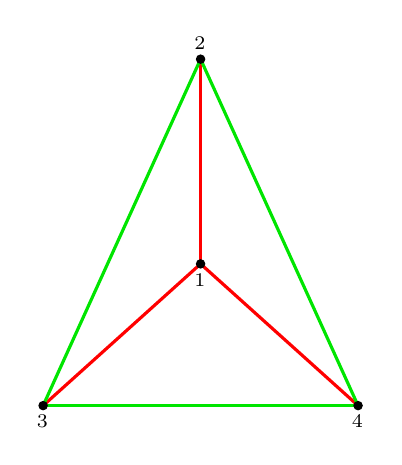
\begin{tikzpicture}
        % coordinates
        \coordinate (x1) at (0,-0.5);
        \coordinate (x2) at (0,2.1);
        \coordinate (x3) at (-2,-2.3);
        \coordinate (x4) at (2, -2.3);
        % boundaries
        \draw[line width=0.4mm, red] (x1) -- (x2);
        \draw[line width=0.4mm, red] (x1) -- (x3);
        \draw[line width=0.4mm, red] (x1) -- (x4);
        \draw[line width=0.4mm, black!10!green] (x2) -- (x3);
        \draw[line width=0.4mm, black!10!green] (x3) -- (x4);
        \draw[line width=0.4mm, black!10!green] (x2) -- (x4);
        
        % vertices
        \filldraw [black] (x1) circle (1.5pt);
        \filldraw [black] (x2) circle (1.5pt);
        \filldraw [black] (x3) circle (1.5pt);
        \filldraw [black] (x4) circle (1.5pt);
        
        % Text
        \node[draw=none, color=black, below] at (x1) {$\x_{1}$};
        \node[draw=none, color=black, above] at (x2) {$\x_{2}$};
        \node[draw=none, color=black, below] at (x3) {$\x_{3}$};
        \node[draw=none, color=black, below] at (x4) {$\x_{4}$};
        
    \end{tikzpicture}
    \label{fig:delta2_1}
    }\hspace{5em}
    \subfloat[$\Delta E^{\triangle}_0$] {    
    \begin{tikzpicture}
        % coordinates
        \coordinate (x1) at (0,-0.5);
        \coordinate (x2) at (0,2.1);
        \coordinate (x3) at (-2,-2.3);
        \coordinate (x4) at (2, -2.3);
        
        % vertices
        \filldraw [black] (x1) circle (1.5pt);
        \filldraw [black] (x2) circle (1.5pt);
        \filldraw [black] (x3) circle (1.5pt);
        \filldraw [black] (x4) circle (1.5pt);
        
        %%%%%%%%%%%%%%%%%%%%%%%%%%%%%%%%%%%%%%%%%%%%%
        % coordinates
        \coordinate (x12) at (x1);
        \coordinate (x22) at ($(x2)!0.3!(x1)$);
        \coordinate (x32) at ($(x3)!0.3!(x1)$);
        \coordinate (x42) at ($(x4)!0.3!(x1)$);
        
        % boundaries
        \draw[line width=0.4mm, red] (x22) -- (x2);
        \draw[line width=0.4mm, red, dashed] (x1) -- (x22);
        \draw[line width=0.4mm, red] (x32) -- (x3);
        \draw[line width=0.4mm, red, dashed] (x1) -- (x32);
        \draw[line width=0.4mm, red] (x42) -- (x4);
        \draw[line width=0.4mm, red, dashed] (x1) -- (x42);
        % boundaries
        \draw[line width=0.4mm, black!10!green, dashed] (x22) -- (x32);
        \draw[line width=0.4mm, black!10!green, dashed] (x32) -- (x42);
        \draw[line width=0.4mm, black!10!green, dashed] (x22) -- (x42);
        
        % vertices
        \filldraw [black] (x12) circle (1.5pt);
        \filldraw [black] (x22) circle (1.5pt);
        \filldraw [black] (x32) circle (1.5pt);
        \filldraw [black] (x42) circle (1.5pt);
        
        % Text
        \node[draw=none, color=black, below] at (x1) {$\x_{1}$};
        \node[draw=none, color=black, above] at (x2) {$\x_{2}$};
        \node[draw=none, color=black, below] at (x3) {$\x_{3}$};
        \node[draw=none, color=black, below] at (x4) {$\x_{4}$};
        
        % Text
        \node[draw=none, color=black, right] at (x22) {$\widetilde{\x}_{2}$};
        \node[draw=none, color=black, below] at (x32) {$\widetilde{\x}_{3}$};
        \node[draw=none, color=black, below] at (x42) {$\widetilde{\x}_{4}$};
        
    \end{tikzpicture}
    \label{fig:delta2_2}
    }
    \caption[Sketch of energies for computing $\Delta^2 E^{\triangle}$]{Sketch of energies for computing $\Delta^2 E^{\triangle}$, see Figure \ref{fig:SE_nucleation2}}
    \label{fig:delta2}
\end{figure}


\subsection{Alternative Nucleation with an Specific Orientation}
\label{sec:alternative_nucleation}

Consider the $\Delta E^{\triangle}$ function from \eqref{eq:Delta_E_Nucleation}.
This definition considers the grain boundary energy function which depends on grains misorientation $\Delta \alpha$ between the nucleated grain and surrounding grains. 
We can choose the orientation of the nucleated grain $\alpha_{\text{nucl}}$ to minimize the energy $E_1^{\triangle}$ of the nucleated grain instead of setting it to zero, that is to find:
\begin{equation}
\min_{\alpha \in [0, 2\pi)} \;\; E_1^{\triangle}.
    \label{eq:minalpha}
\end{equation}
It is preferable a fast algorithm to approximate \eqref{eq:minalpha} rather than an expensive solver that finds the exact minimum since each vertex will execute the same procedure, even if the search is performed in parallel. 
A simple procedure is to obtain an approximation to the minimum. 
We define the orientation of the nucleated grain as $\alpha_{\text{nucl}}$ to be an approximation to \eqref{eq:minalpha}.
The algorithm consists in generate a sample of values in the range $[0, 2\pi]$ and evaluate $E_1^{\triangle}$ and find the value that yields the minimum energy.
%Numerical simulation can be observed in Figure~\ref{fig:SEnucl2_evolution}

\section{Stored Energy Vertex Model with Nucleation Algorithm}

The algorithm of this model considers first the computation of boundaries properties such as arc lengths and energies and the computation of grain areas. 
We choose to perform continuous nucleation, that is, nucleating at regular intervals of the simulation. 
In our case we choose to nucleate at each time step a single grain as seen in~\cite{raabe2006continuum}. 
Therefore we choose a suitable site for nucleation as studied in previous sections considering the site with the lowest nucleation factor $\Delta^2E^{\triangle}$. 
If there is a site for nucleation the grain is added and neighboring topology is updated along with their related modified quantities, that is, recompute arc lengths, energies and areas. 
The next stage considers the computation of the vertices velocities using the matrix-free approach described in Section~\ref{sec:se_numerical}. Then, extinction times for each boundary are computed and we label boundaries that will flip, that is when $t_{\text{ext}} \in[0,\Delta t]$. 
Here we must decide which flippings are safe to perform and therefore we avoid  neighbor transitions. 
The algorithm to avoid this is explained in Chapter~\ref{chap:parallelflip}.
This model may generate configurations of two grains of three sides, we detect them and remove them if any of the boundaries related will flip. 
We also remove in this stage any three sided grain that will have a boundary marked as flip. 
After this fixes we apply the remaining flippings, we update the vertices positions and the system evolves to the time $t+\Delta t$. Algorithm \ref{alg:storedenergy} summarizes the described algorithm.

\begin{algorithm}[t]
\caption{Stored Energy Vertex Model}
\label{alg:storedenergy}
\begin{algorithmic}[1]
\Procedure{SEVM}{$n_\text{iters}$}
\State $(t, n_\text{iters}) \gets (0, 0)$

\EndProcedure
\end{algorithmic}
\end{algorithm}

\section{Numerical Experiments}

Numerical experiments were performed using \numprint{100000} initial grains. 
Grain boundary energy anisotropy is added by using $\eqref{eq:gamma}$ with parameters $\varepsilon = \{0.02, 0.2\}$. 
The initial distribution of stored energy is chosen to propitiate more grains with high values of stored energies and thus more places for nucleation. 
We use a triangular distribution for this purpose with the following parameters:
\begin{equation}
    \SE \thicksim \text{Triangular}(3,6,6)
    \label{eq:triangular_dist}
\end{equation}
where $\SE = 6$ is chosen due to previous study in Section~\ref{sec:dynamics} (see Figure~\ref{fig:SE_experiments} and numerical experiments related). 
Figure~\ref{fig:SE_se_0} shows the triangular distribution. 
The computational domain is $\Omega = [0,15]^2$ with periodic boundary conditions.

Notice, since the bound for maximum difference of
stored energy is an absolute value (it is $6$), 
we needed to increase the computational domain
so we were able to obtain $\Delta^2 E^{\triangle}<0$,
otherwise this is very unlikely.
If this constraint is not satisfied,
we have have triple junctions with dihedral
angles greater that $\pi$ and
those triple junctions could cross grain
boundaries and create a corrupt grain
network. 
This may be handled with different
types of topological transition, see \cite{pikekos2008stochastic}.

Stages of the numerical simulation with the two explained nucleation variations can be observed in Figures~\ref{fig:SE_evolution} and~\ref{fig:SEnucl2_evolution}. 
Both experiments were run using $\varepsilon = 0.02$

% Here speak about statistics
\subsection{Energy Minimization}
Figure~\ref{fig:SE_energies_1} shows energy curves over time for various initial conditions of grain networks following the formula \eqref{eq:SEtotalenergy} with $\varepsilon = 0.2$ to make more noticeable the effect of the grain boundary energy. 
The stored energy algorithms used were the following: No nucleation, which is a Vertex model with stored energy, nucleation choosing sites with orientation $\alpha = 0$ and nucleation choosing sites with orientation $\alpha = \alpha_{\text{nucl}}$.

The Stored Energy models shows some interesting behaviors. 
At the first time steps the three models behave very similar, minimizing the overall energy. Near $t = 0.6$ the nucleating models actually induces some small energy increments with respect to the no nucleation model but they are very small with respect to the magnitude of the total energy but still appreciable since both associated families of curves are above the family of curves corresponding to the no nucleation model. 
This behavior can be seen in the highlighted zone in Figure~\ref{fig:SE_energies_1}. 
A zoom of this behavior is shown in Figure~\ref{fig:SE_energies_2} where both nucleating models are more energetic until $t \approx 1$.

At some point near $t = 1$ nucleating models starts to minimize the energy faster than the no nucleating model. 
The nucleation model using $\alpha = 0$ does not minimize the energy as fast the nucleation model using $\alpha_{\text{nucl}}$, which is caused by greedy choice of the best possible $\alpha$ for nucleation. 
This greedy choice does not guarantee obtaining the minimum configuration of energy at later stages of the numerical simulation. 
In fact near $t = 1.6$ the model with nucleation using $\alpha = 0$ reaches faster a minimum energy than using $\alpha_{\text{nucl}}$, which is explained by the fact that after the recrystallization process - where there are not possible sites for nucleating - and the new stage of grain growth one model has an isotropic configuration since all orientations are equal and thus the misorientation is zero yielding $\gamma^{(k)} = 1$, and the other model reaches an anisotropic configuration which naturally has more energy since grains are misaligned.

\begin{figure}[t]
    \centering
    \subfloat[System energy (normalized) over time for different models of stored energy.]{
        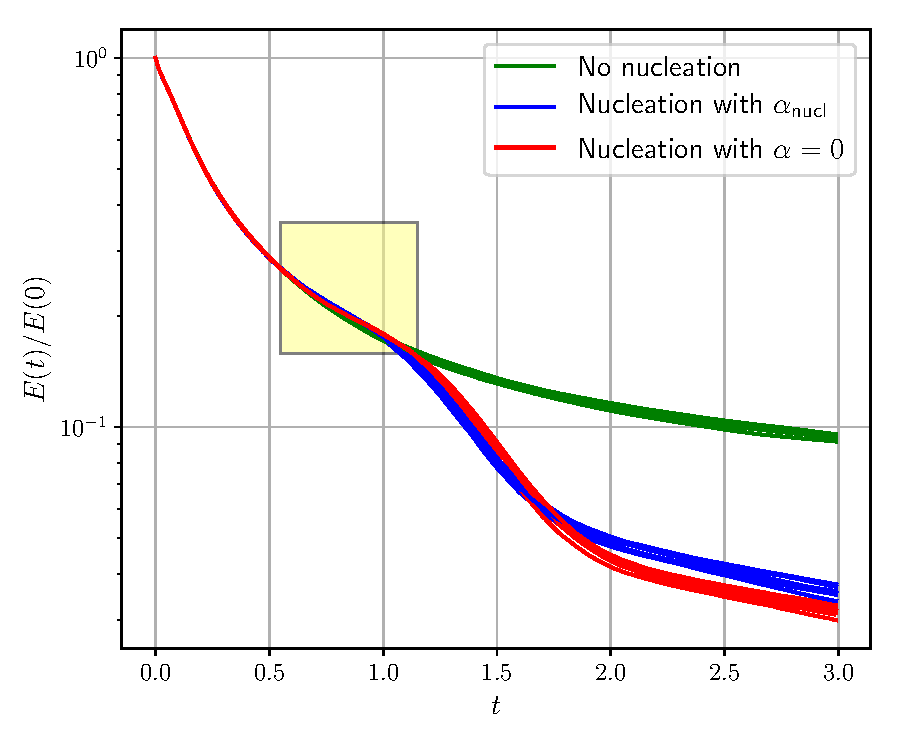
\includegraphics[scale=0.45]{figures/stored_energy/SE_energy.pdf}
        \label{fig:SE_energies_1}
    }%
    \hspace{1em}
    \subfloat[Zoom of the first nucleation stage where energy is added to the system over non-nucleating model simulations.
    Yellow square in Figure on the left side.]{
        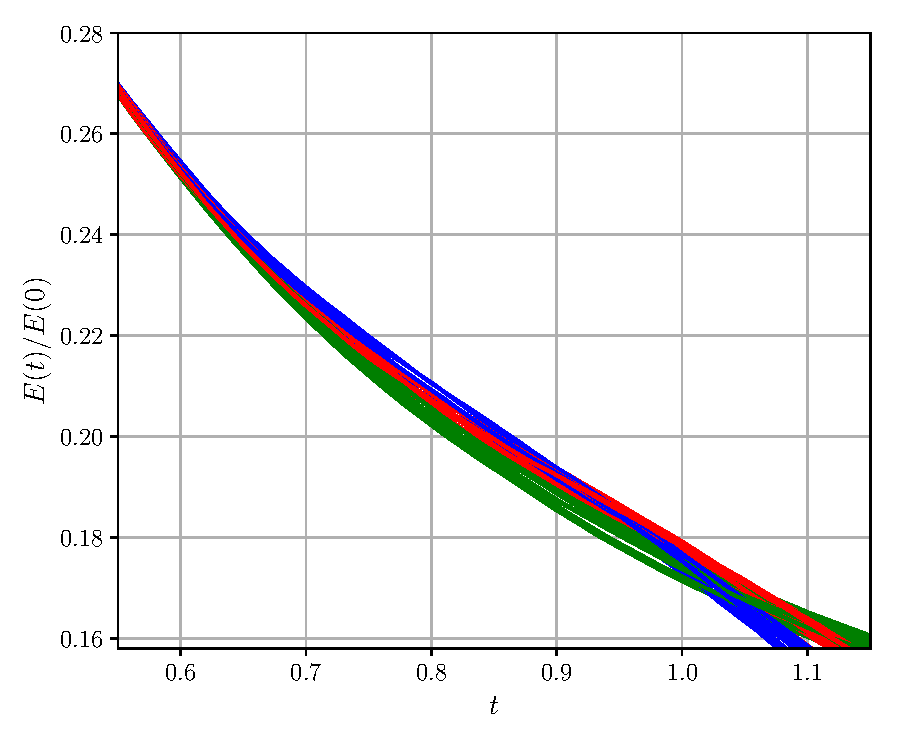
\includegraphics[scale=0.45]{figures/stored_energy/SE_energy_zoom.pdf}
        \label{fig:SE_energies_2}
    }
    \caption{System energy over time for different models of stored energy.}
    \label{fig:SE_energies}
\end{figure}

\subsection{Statistics from Model with Basic Nucleation}
\label{sec:stats_basicnucl}

Figure~\ref{fig:SE_evolution} shows the stages observed in the numerical simulation. Figure~\ref{fig:SE_dist_0} is a zoom of the initial condition with \numprint{100000} grains generated via Voronoi tessellation. 
Figure~\ref{fig:SE_dist_1} shows first nucleations in the grain network. Those grains are initialized with $\SE = 0$ and $\alpha = 0$. After some time the nucleated grains will start to increase its number of sides as seen in Figure~\ref{fig:SE_dist_2}. Finally, Figure~\ref{fig:SE_dist_3} shows a fully recrystallized grain network. Under the mentioned parameters this network will evolve ruled by isotropic vertex model naturally since $\Delta \alpha = 0$ for every boundary (and thus $\gamma^{(k)} = 1$) and the energy of the system becomes:
\begin{equation}
    E = \sum_{k=1}^K \AL_k.
    \label{eq:vertex_energy}
\end{equation}

\begin{figure}[ht]
    \centering
    %\hspace{-4.5em}
    \subfloat[Zoom of Initial distribution generated via Voronoi tessellation.]{
    \includegraphics[scale=0.40, trim={2em 0 2em 0}]{figures/stored_energy/SE/snaps/000000.pdf}
    \label{fig:SE_dist_0}
    }%
    \subfloat[First nucleations.]{
    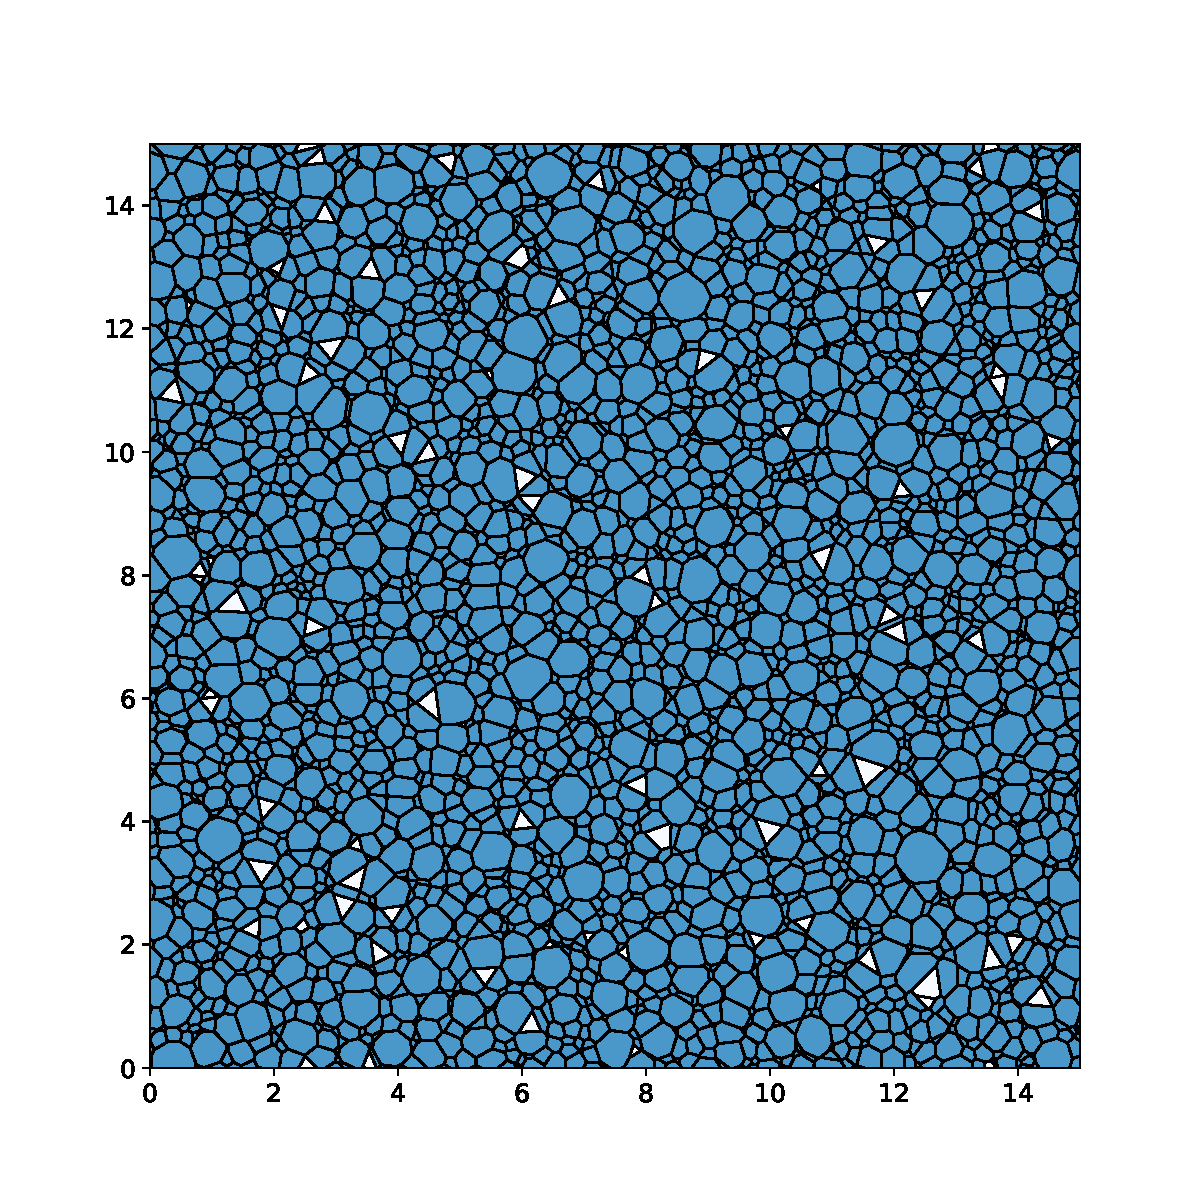
\includegraphics[scale=0.40, trim={2em 0 2em 0}]{figures/stored_energy/SE/snaps/000070.pdf}
    \label{fig:SE_dist_1}
    }\\%
    %\hspace{-4.5em}
    \subfloat[Nucleation stage.]{
    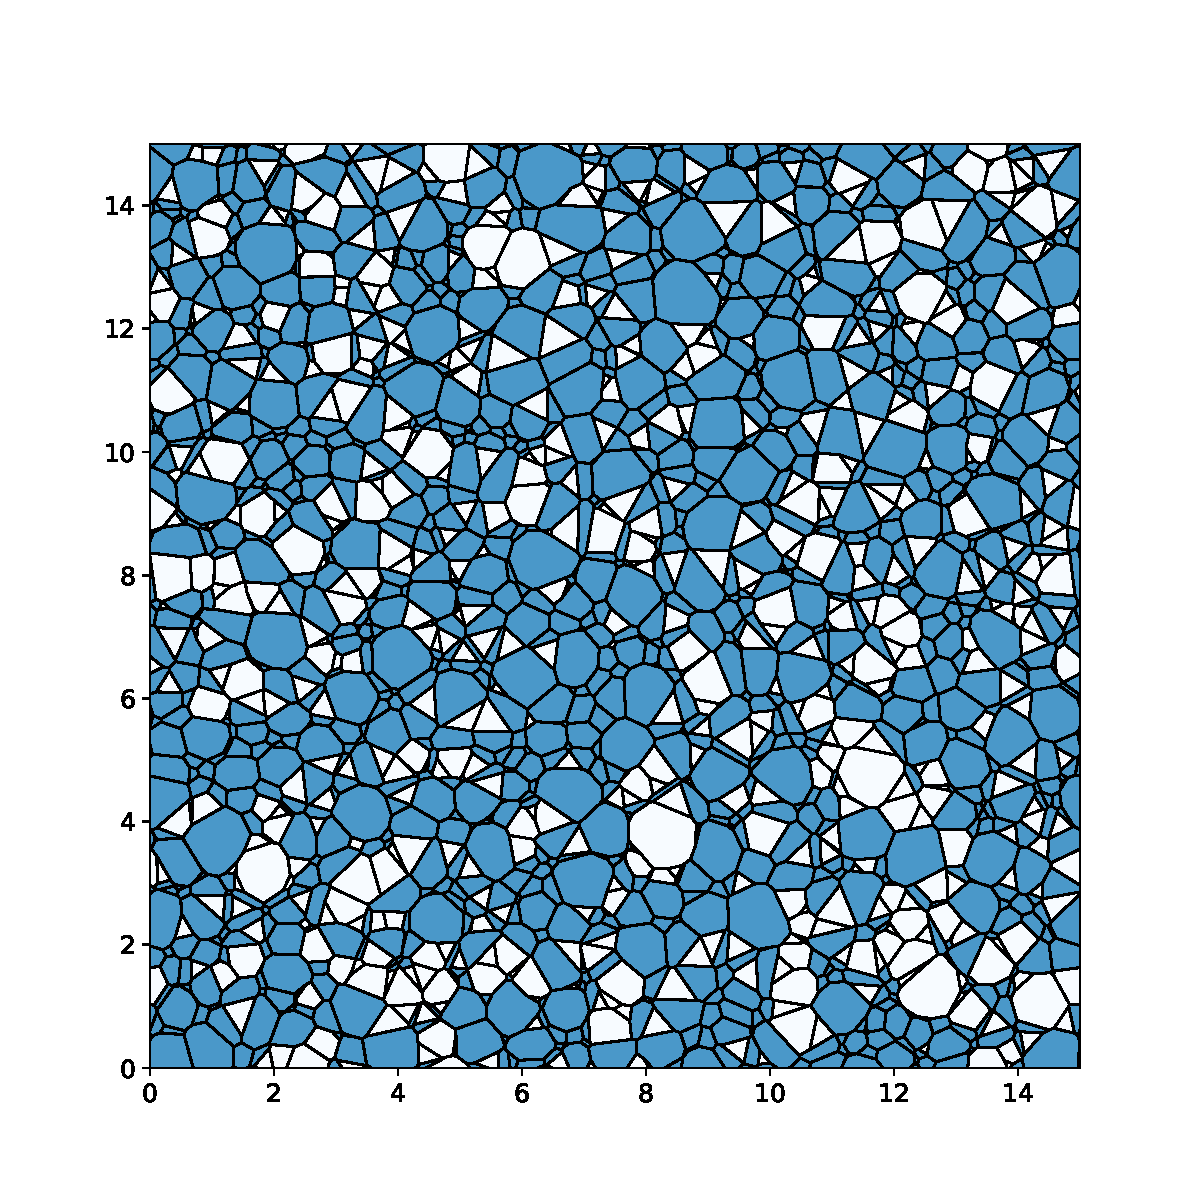
\includegraphics[scale=0.40, trim={2em 0 2em 0}]{figures/stored_energy/SE/snaps/000110.pdf}
    \label{fig:SE_dist_2}
    }%
    \subfloat[Recrystallization.]{
    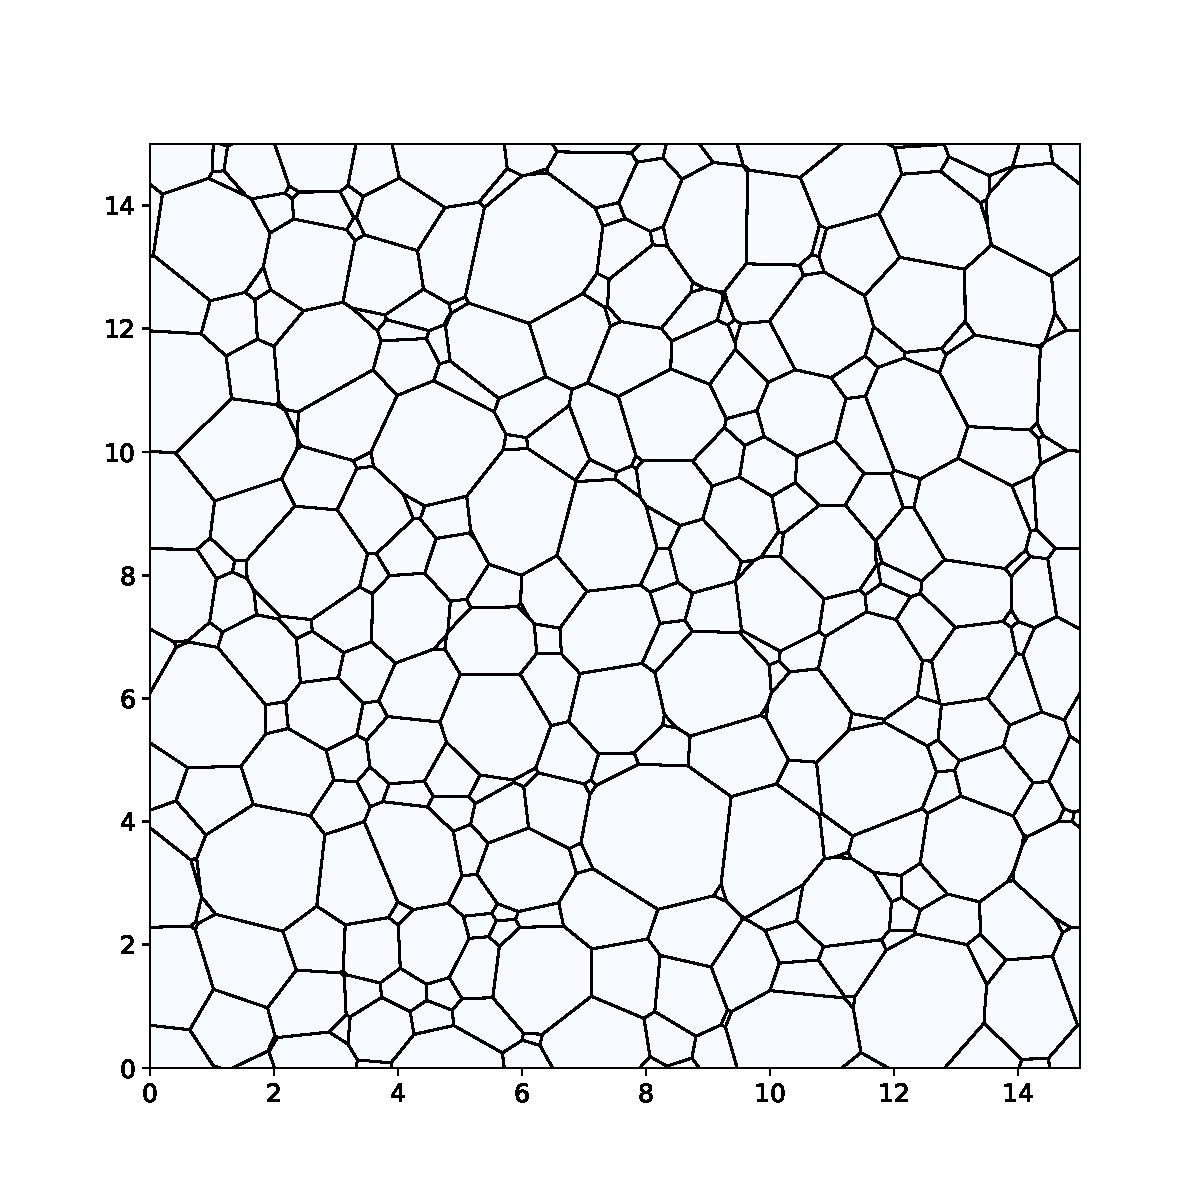
\includegraphics[scale=0.40, trim={2em 0 2em 0}]{figures/stored_energy/SE/snaps/000240.pdf}
    \label{fig:SE_dist_3}
    }%
\caption{Stages of grain network evolution nucleating with $\alpha = 0$.}
    \label{fig:SE_evolution}
\end{figure}

Statistics extracted for each of the stages are shown in Figures~\ref{fig:SE_areas}, \ref{fig:SE_dihedral},  \ref{fig:SE_gbcd} ,\ref{fig:SE_nsides} and~\ref{fig:SE_se}.  We begin describing relative area distribution from Figure~\ref{fig:SE_areas} in both linear and logarithmic scale. From now on we choose three representative experiments per stage based on the first bin of the linear scale distribution. First experiment is related to the largest first bin (in blue), second experiment is related to the median of the first bin (in red) and third experiment is related to the shortest first bin (in green).

Figure~\ref{fig:SE_areas_0} shows the initial condition distribution. Figure~\ref{fig:SE_areas_1} shows the distribution during the first nucleations, which is resembles the Vertex model tail in the log scale distribution related to a great quantity of small grains. Figure~\ref{fig:SE_areas_2} and~\ref{fig:SE_areas_3} shows a slightly reduce in the number of small grains but in overall the shape of the distribution remains the same.

\begin{figure}[ht]
    \vspace{-1em}
    \centering
    \subfloat[Initial condition.]{
    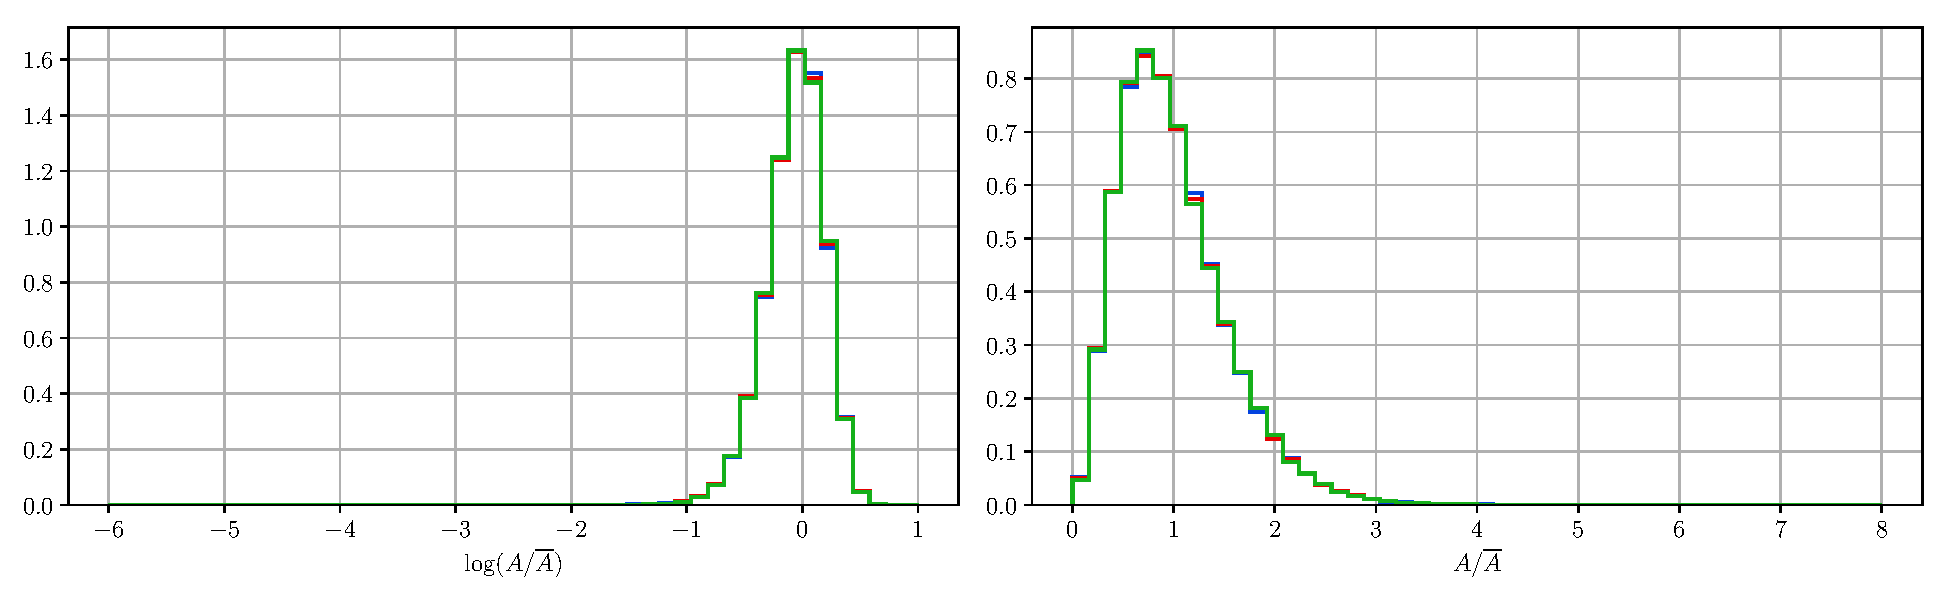
\includegraphics[scale=0.42, trim={0em 1em 0em 2em}]{figures/stored_energy/SE/areas/000000_nuclconstant_set.pdf}
    \label{fig:SE_areas_0}
    }\\
    \subfloat[First nucleations.]{
    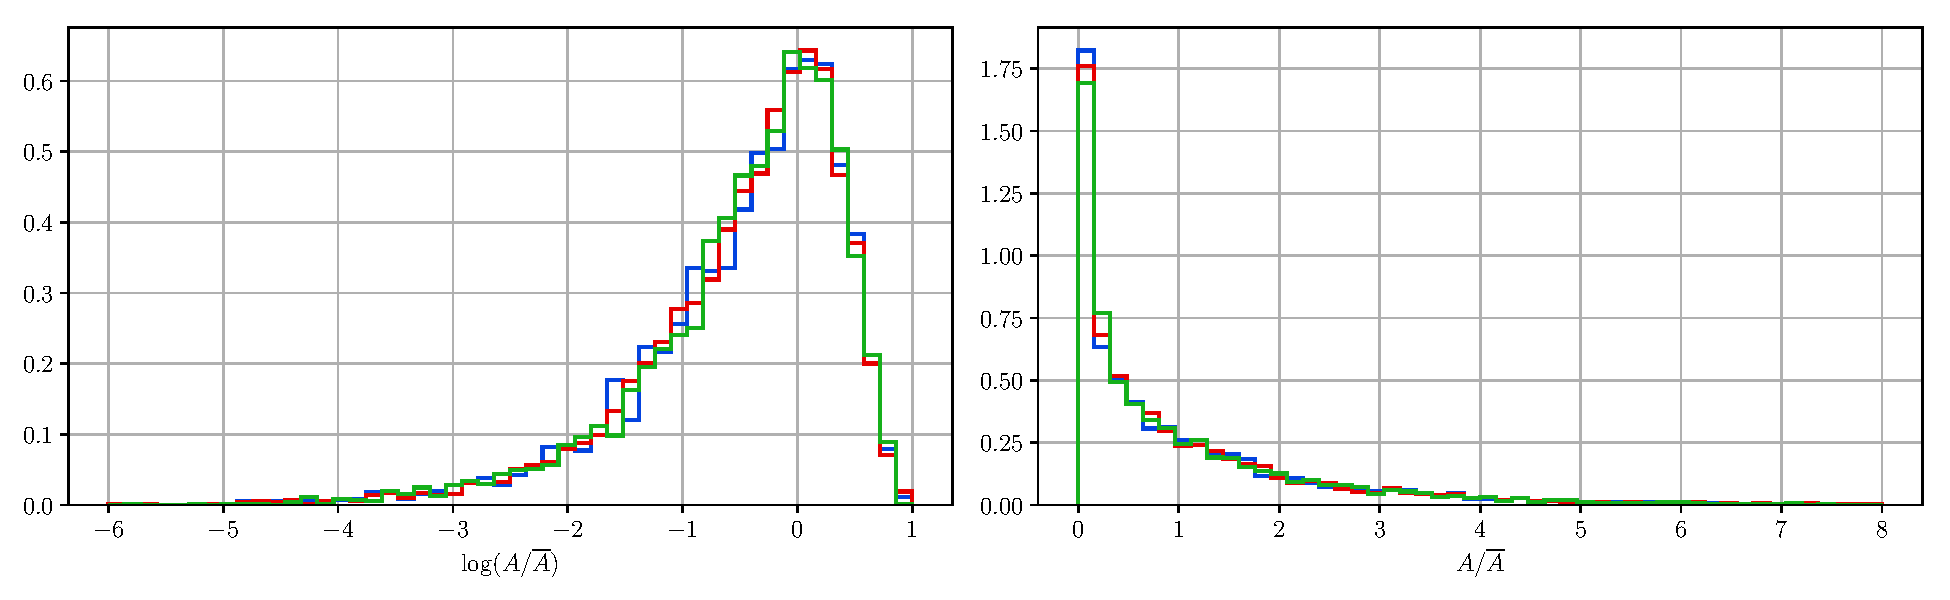
\includegraphics[scale=0.42, trim={0em 1em 0em 2em}]{figures/stored_energy/SE/areas/000070_nuclconstant_set.pdf}
    \label{fig:SE_areas_1}
    }\\%
    %\hspace{-4.5em}
    \subfloat[Nucleation stage.]{
    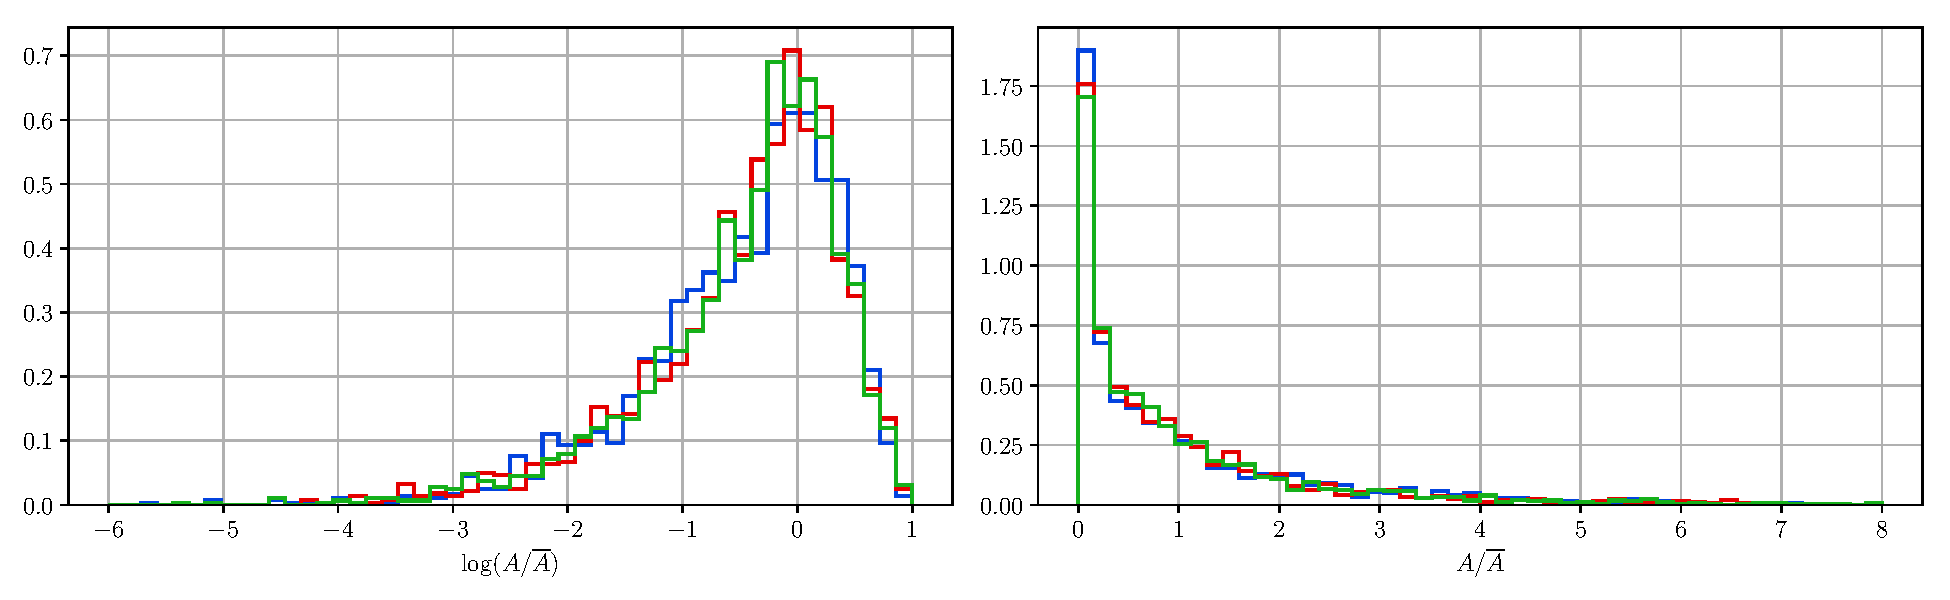
\includegraphics[scale=0.42, trim={0em 1em 0em 2em}]{figures/stored_energy/SE/areas/000110_nuclconstant_set.pdf}
    \label{fig:SE_areas_2}
    }\\%
    \subfloat[Recrystallization.]{
    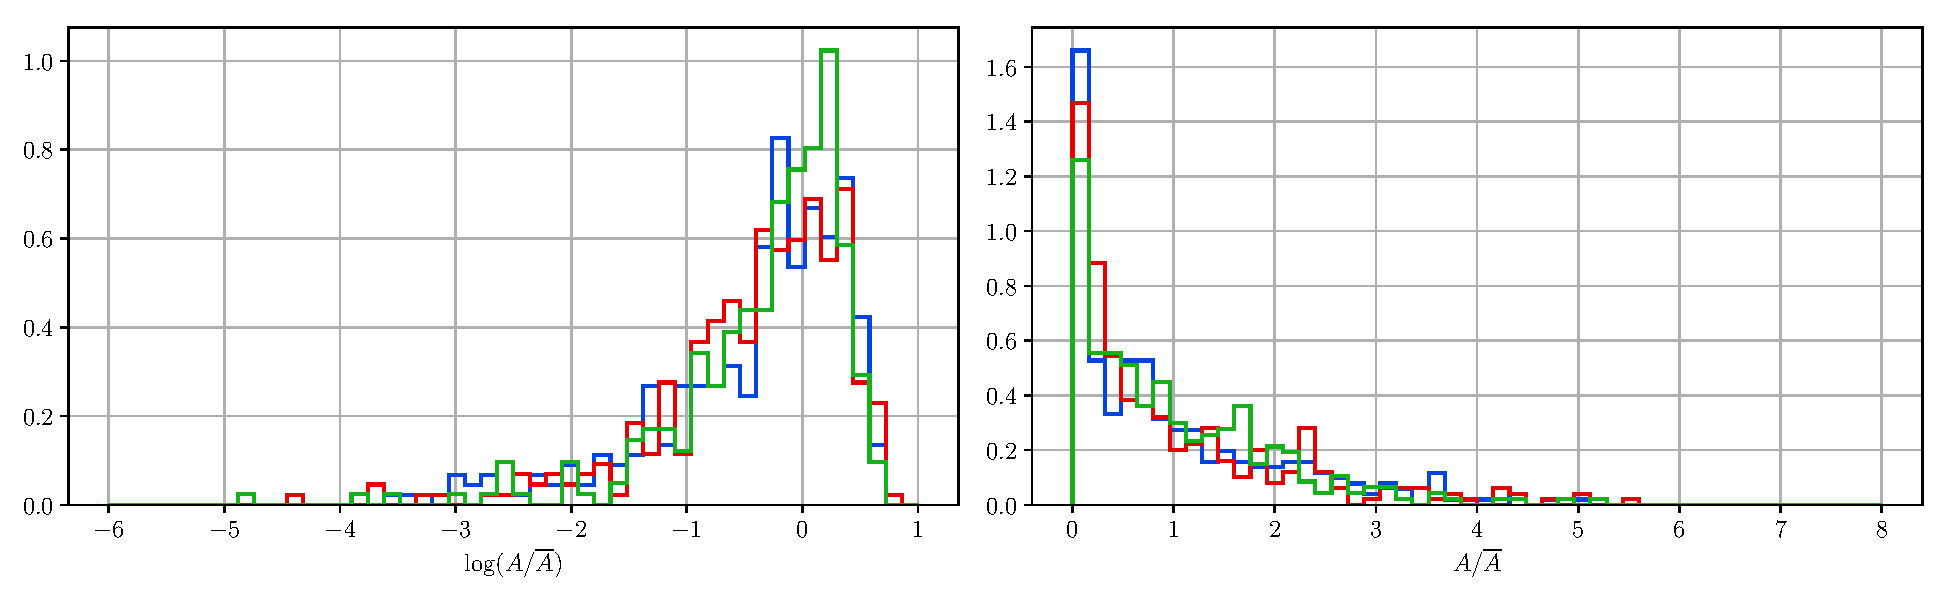
\includegraphics[scale=0.42, trim={0em 1em 0em 2em}]{figures/stored_energy/SE/areas/000240_nuclconstant_set.pdf}
    \label{fig:SE_areas_3}
    }%
    \caption{Grain relative area distributions at different stages of grain network evolution and nucleation with $\alpha = 0$.}
    \label{fig:SE_areas}
\end{figure}


Figure~\ref{fig:SE_dihedral_0} shows the distribution of dihedral angle of the initial condition. Figure~\ref{fig:SE_dihedral_1} shows the distribution during the stage of first nucleations. The distribution is regular as expected since before this stage only grain growth has occurred and there is also a shift to bigger angles from the steady state dihedral angle of $2\pi/3$. Figure~\ref{fig:SE_dihedral_2} shows the distribution when the nucleation stage has generated a lot of new grains. 
This creates a bimodal distribution of small angles and therefore the angles greater than $\pi$ has also increased. 
This can be related to the existence of large grains as seen in Figure~\ref{fig:SE_dist_2}. Finally, Figure~\ref{fig:SE_dihedral_3} shows the dihedral distribution angle after full recrystallization which is very similar as the obtained in the early grain growth stage prior to nucleations.

\begin{figure}[ht]
    \centering
    \subfloat[Initial condition.]{
    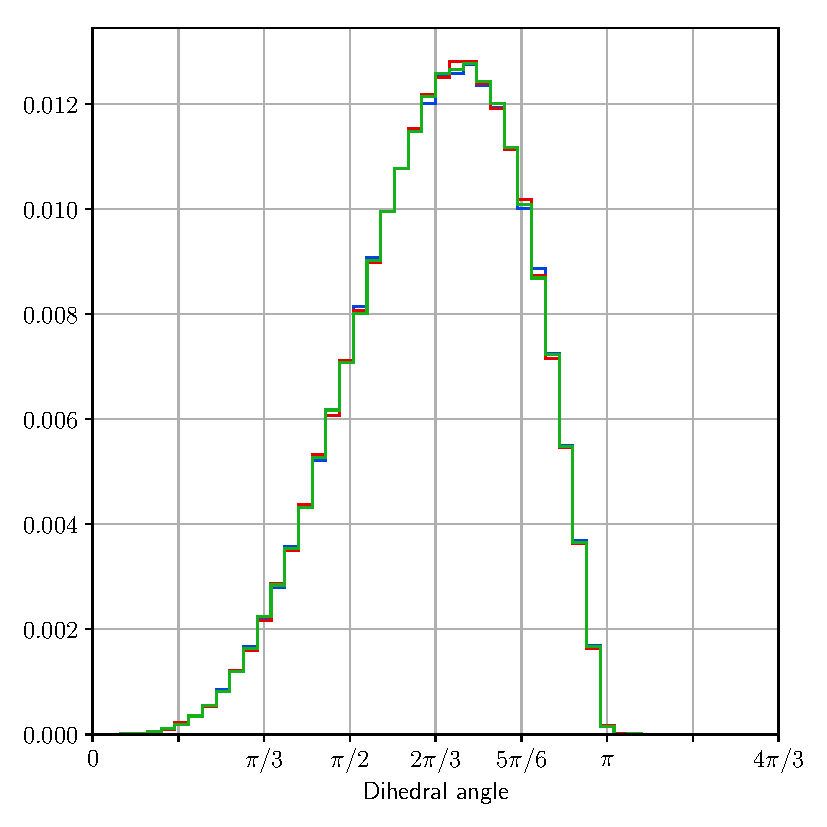
\includegraphics[scale=0.45, trim={0em 0 0em 0}]{figures/stored_energy/SE/dihedral/000000_nuclconstant_set.pdf}
    \label{fig:SE_dihedral_0}
    }%
    \subfloat[First nucleations.]{
    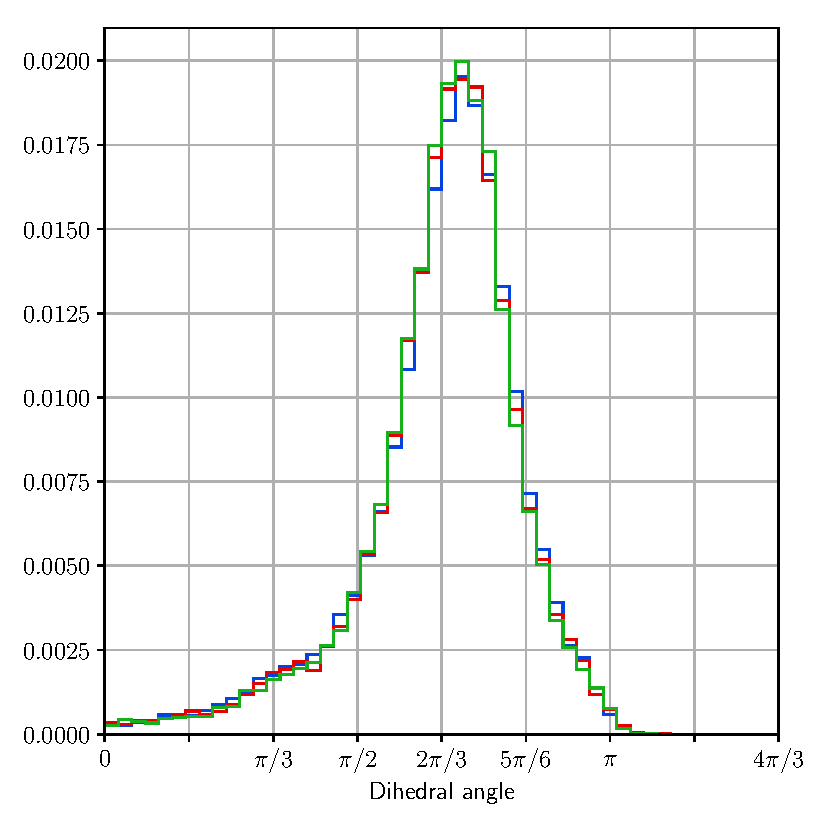
\includegraphics[scale=0.45, trim={0em 0 0em 0}]{figures/stored_energy/SE/dihedral/000070_nuclconstant_set.pdf}
    \label{fig:SE_dihedral_1}
    }\\%
    %\hspace{-4.5em}
    \subfloat[Nucleation stage.]{
    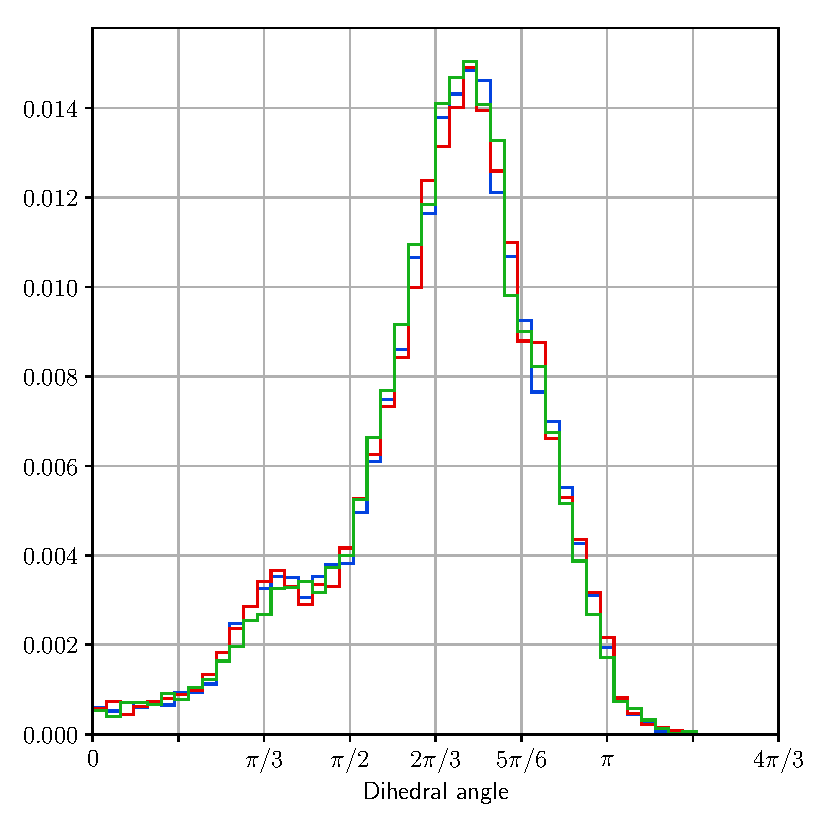
\includegraphics[scale=0.45, trim={0em 0 0em 0}]{figures/stored_energy/SE/dihedral/000110_nuclconstant_set.pdf}
    \label{fig:SE_dihedral_2}
    }%
    \subfloat[Recrystallization.]{
    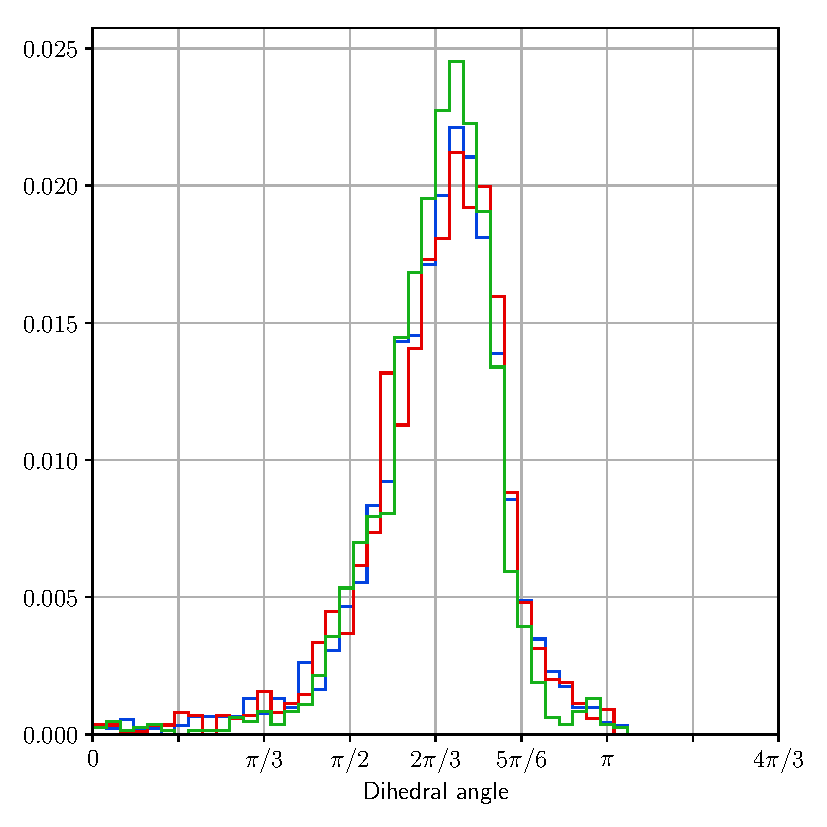
\includegraphics[scale=0.45, trim={0em 0 0em 0}]{figures/stored_energy/SE/dihedral/000240_nuclconstant_set.pdf}
    \label{fig:SE_dihedral_3}
    }%
\caption{Dihedral angle distributions at different stages of grain network evolution and nucleation with $\alpha = 0$.}
    \label{fig:SE_dihedral}
\end{figure}

Grain boundary character distribution (GBCD) is shown in Figure~\ref{fig:SE_gbcd}. 
Dark blue continuous line in background shows the grain boundary energy function from \eqref{eq:gamma} which is
\begin{equation*}
    \gamma(\Delta \alpha ) = 1+\frac{\varepsilon}{2}\left(1 - \cos^3(4 \Delta \alpha) \right).
\end{equation*}
We present the GBCD in two plots. One is the measured misorientation in $[-\pi/4, \pi/4)$ at the left of Figure~\ref{fig:SE_gbcd} and at the right a symmetric version of the GBCD which accumulates the misorientations by symmetry in $[0,\pi/4)$.

The GBCD of initial condition is shown in Figure~\ref{fig:SE_gbcd_0}. Notice that the misorientations are distributed uniformly over $[-\pi/4, \pi/4)$.  Figure~\ref{fig:SE_gbcd_1} shows a perturbation in the initial distribution towards $\Delta \alpha = 0$ and the tendency to form minimum at $\pm \pi/4$. %The nucleated grains affect the distribution delaying some effect expected from the energy function at the critical points $\pm \pi/4$ and $0$.
Figure~\ref{fig:SE_gbcd_2} shows the GBCD at nucleation stage. Since the nucleated grains have orientation zero, the middle bin grows accumulating all the data, the entire grain network is evolving towards an isotropic state. In Figure~\ref{fig:SE_gbcd_3} the final distribution is shown after full recrystallization. Notice that all orientations have become zero and thus an isotropic regime is reached, the GBCD becomes a single bin at misorientation zero.

\begin{figure}[ht]
    \centering
    \subfloat[Initial condition.]{
    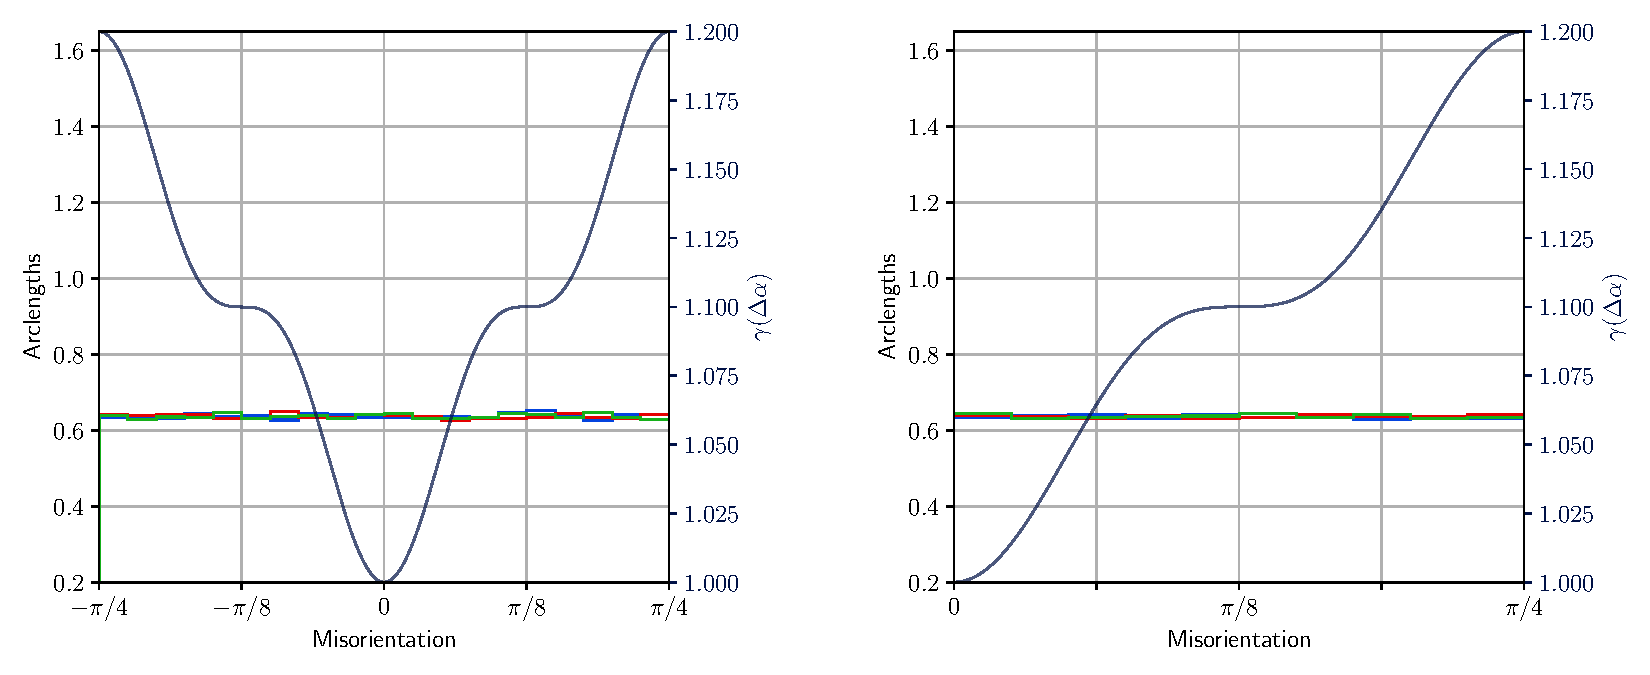
\includegraphics[scale=0.5, trim={0em 0 0em 0em}]{figures/stored_energy/SE/gbcd/000000_nuclconstant_set.pdf}
    \label{fig:SE_gbcd_0}
    }\\
    \subfloat[First nucleations.]{
    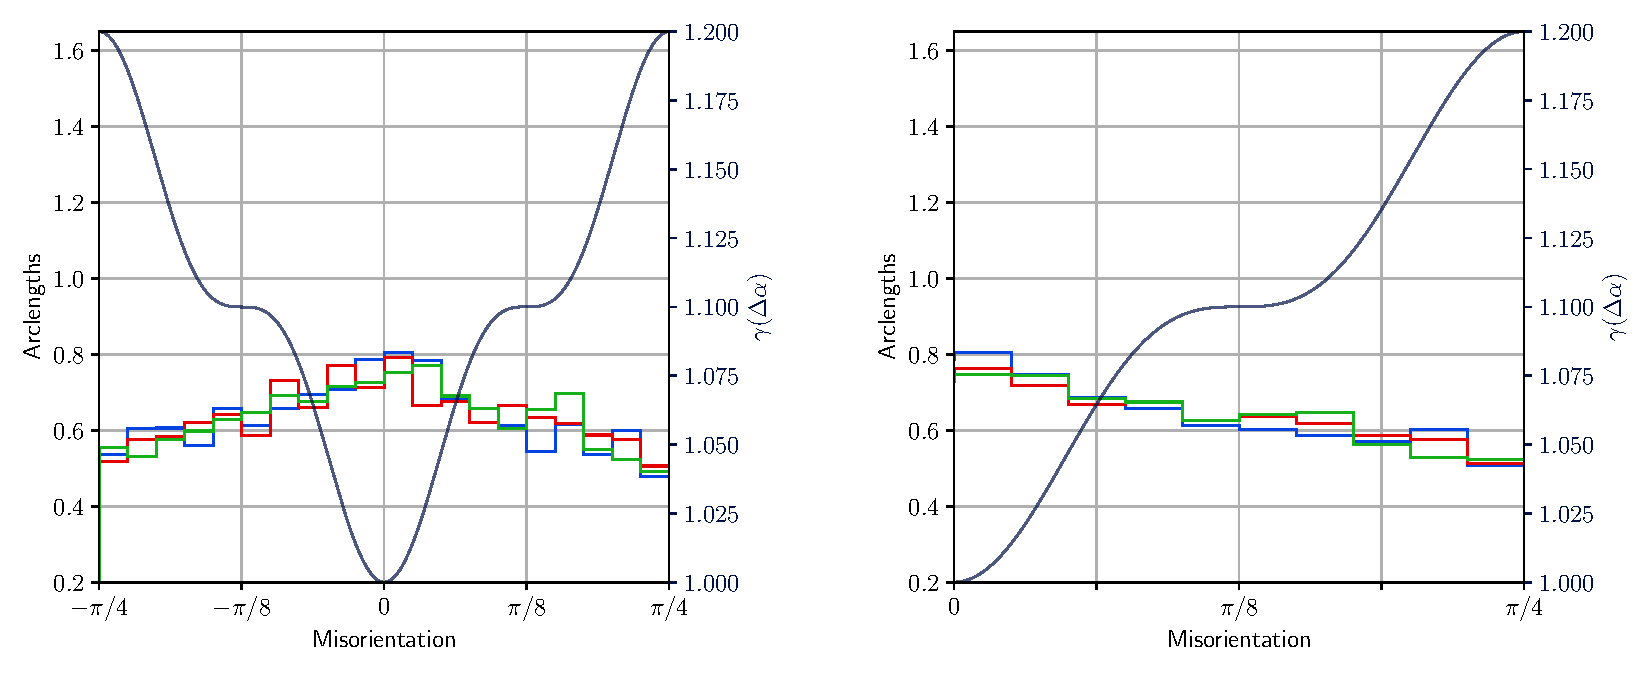
\includegraphics[scale=0.5, trim={0em 0 0em 0em}]{figures/stored_energy/SE/gbcd/000070_nuclconstant_set.pdf}
    \label{fig:SE_gbcd_1}
    }
    \caption{Grain Boundary Character distributions at different stages of grain network evolution and nucleation with $\alpha = 0$.}
\end{figure}
\begin{figure}[ht]\ContinuedFloat
    \centering
    \subfloat[Nucleation stage.]{
    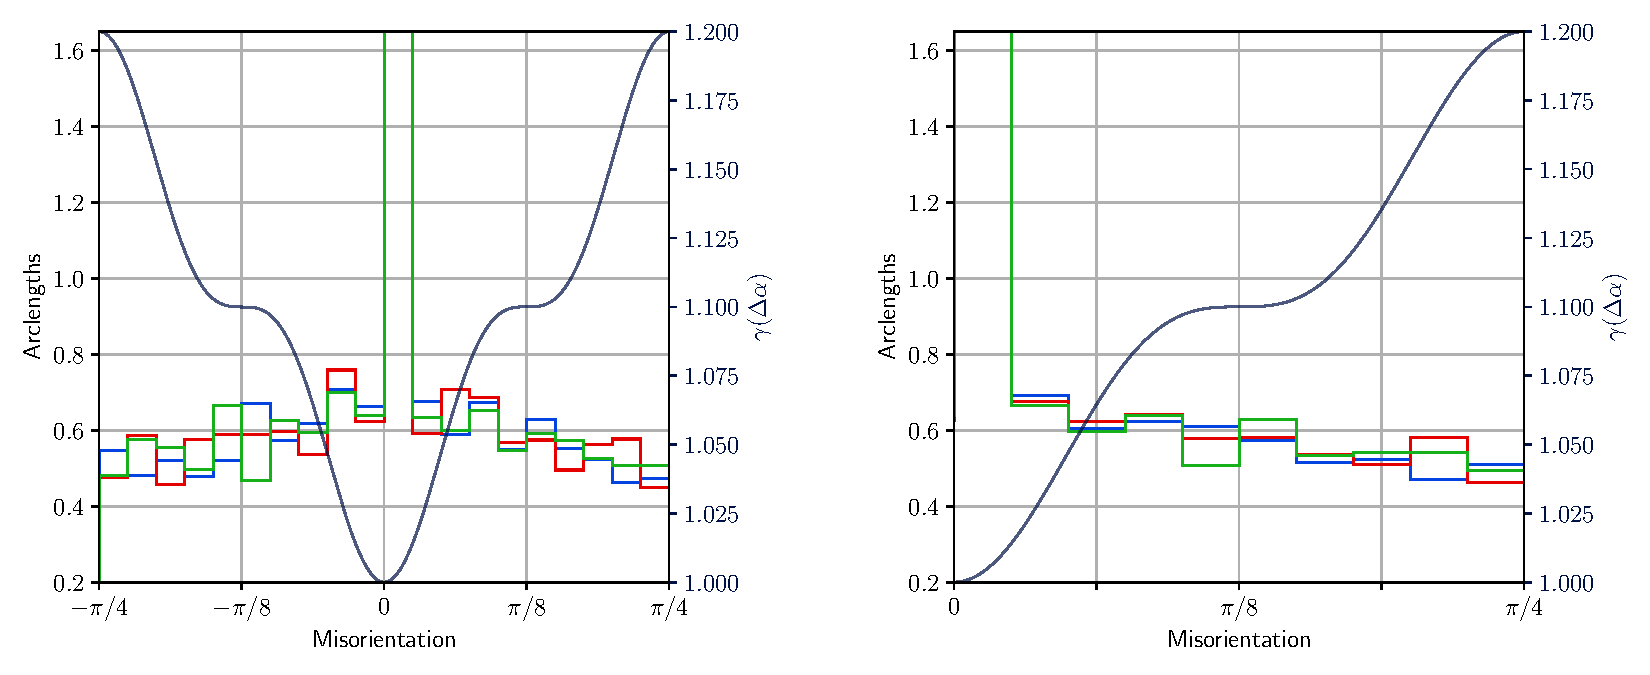
\includegraphics[scale=0.5, trim={0em 0 0em 0em}]{figures/stored_energy/SE/gbcd/000110_nuclconstant_set.pdf}
    \label{fig:SE_gbcd_2}
    }\\
    \subfloat[Recrystallization.]{
    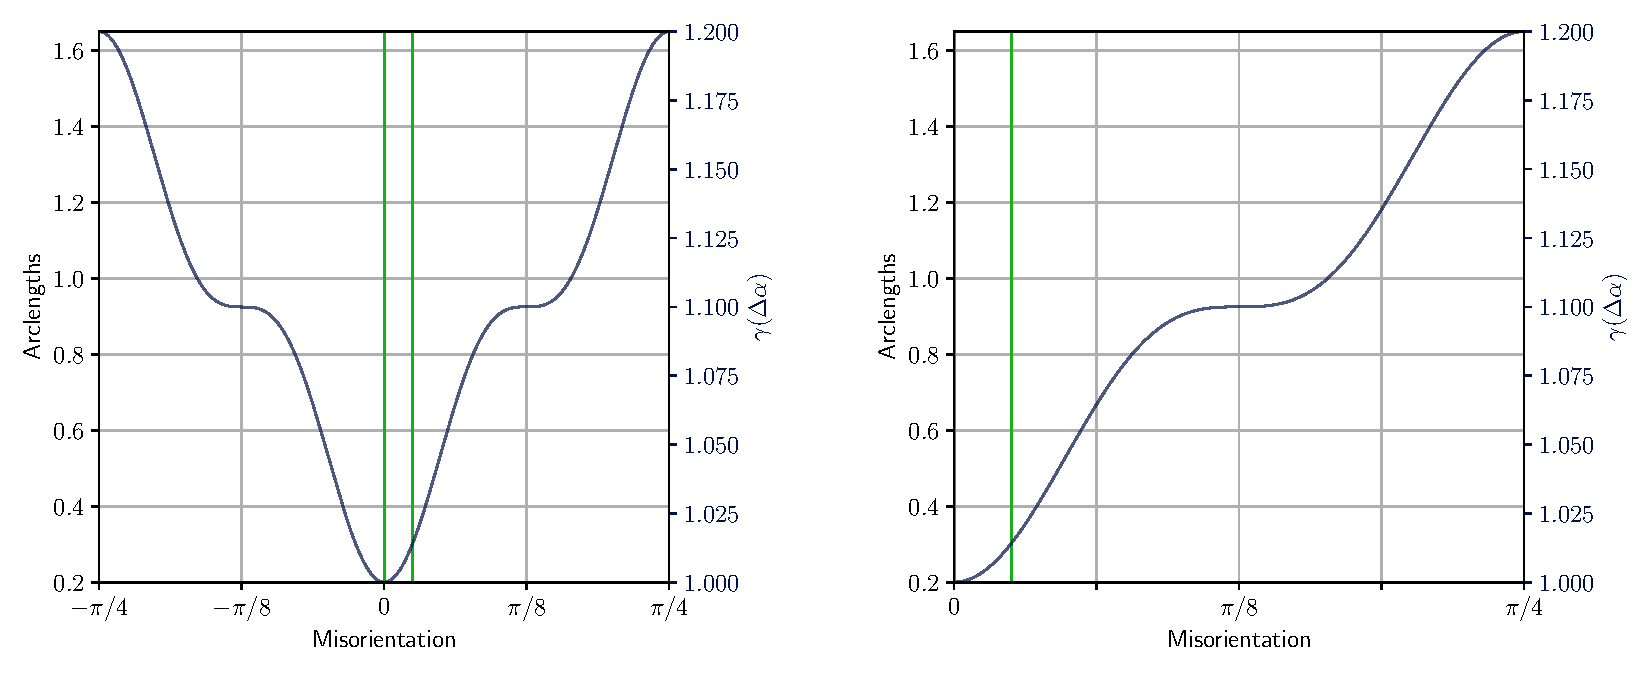
\includegraphics[scale=0.5, trim={0em 0 0em 0em}]{figures/stored_energy/SE/gbcd/000240_nuclconstant_set.pdf}
    \label{fig:SE_gbcd_3}
    }%
    \caption{Grain Boundary Character distributions at different stages of grain network evolution and nucleation with $\alpha = 0$. (Cont.)}
    \label{fig:SE_gbcd}
\end{figure}

Distribution of average number of sides is shown in Figure~\ref{fig:SE_nsides}. Figure~\ref{fig:SE_nsides_1} shows the initial condition distribution, where the mode is at six, which means that the most frequent grains are six sided. 
After grain growth and during first nucleations the mode changes to five and we observe many small grains, mostly three sided grains, as seen in Figure~\ref{fig:SE_nsides_2}. 
During nucleation regime the mode in fact is three because nucleated grains are from this class. Also the frequency of four sided increases. This may be explained since they were formerly nucleated three sided grains that may have increased their number of sides if a nucleation happened in one of their vertex. We observe that huge grains exists but they are not determined to stay forever. Finally in Figure~\ref{fig:SE_nsides_3} after fully recrystrallization the distribution stabilizes and three sided grains are again of low frequency, the mode also returns to be five.

\begin{figure}[ht]
    \centering
    \subfloat[Initial condition.]{
    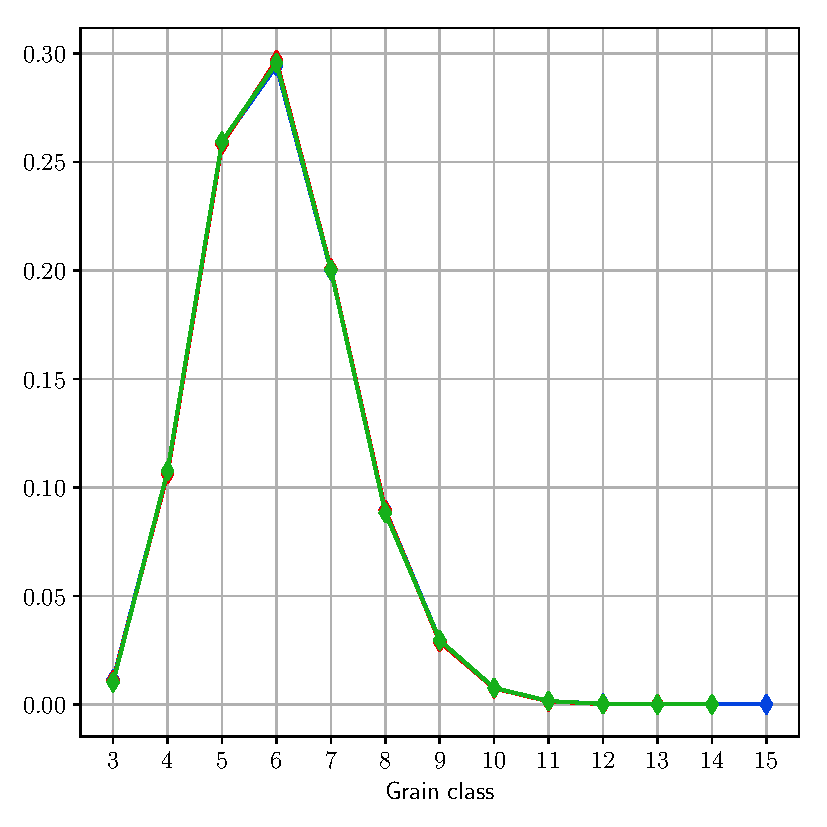
\includegraphics[scale=0.45, trim={0em 0 0em 0}]{figures/stored_energy/SE/nsides/000000_nuclconstant_set.pdf}
    \label{fig:SE_nsides_0}
    }%
    \subfloat[First nucleations.]{
    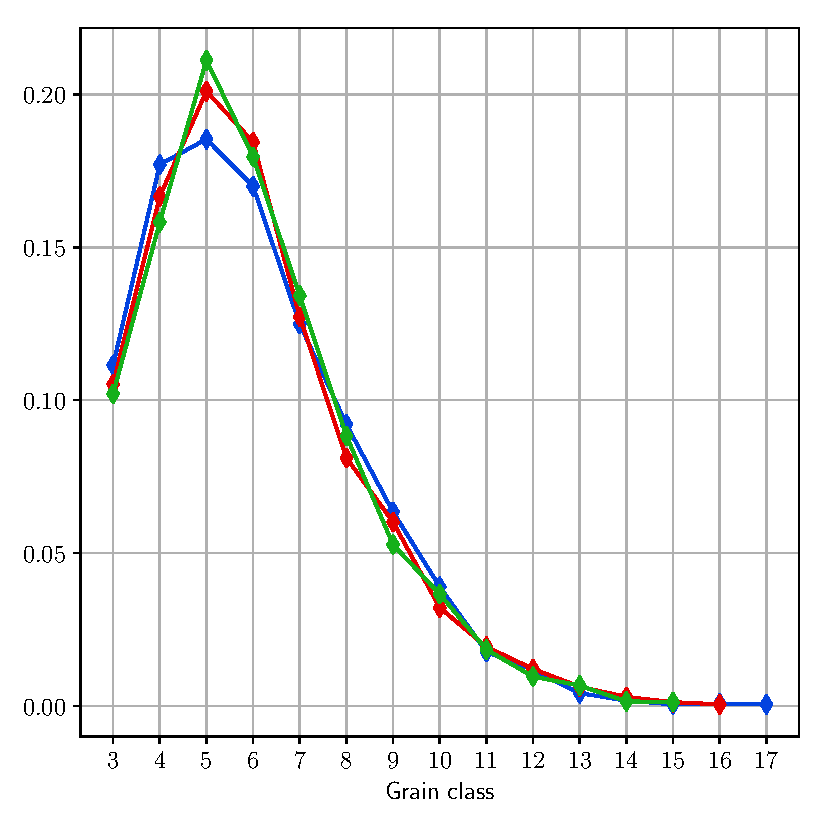
\includegraphics[scale=0.45, trim={0em 0 0em 0}]{figures/stored_energy/SE/nsides/000070_nuclconstant_set.pdf}
    \label{fig:SE_nsides_1}
    }\\%
    %\hspace{-4.5em}
    \subfloat[Nucleation stage.]{
    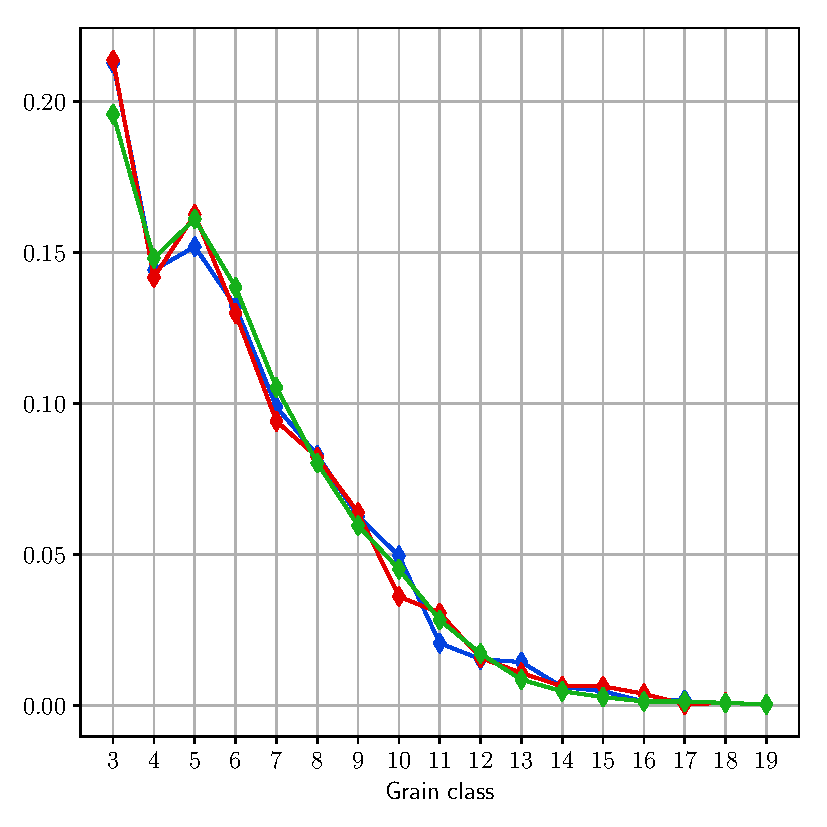
\includegraphics[scale=0.45, trim={0em 0 0em 0}]{figures/stored_energy/SE/nsides/000110_nuclconstant_set.pdf}
    \label{fig:SE_nsides_2}
    }%
    \subfloat[Recrystallization.]{
    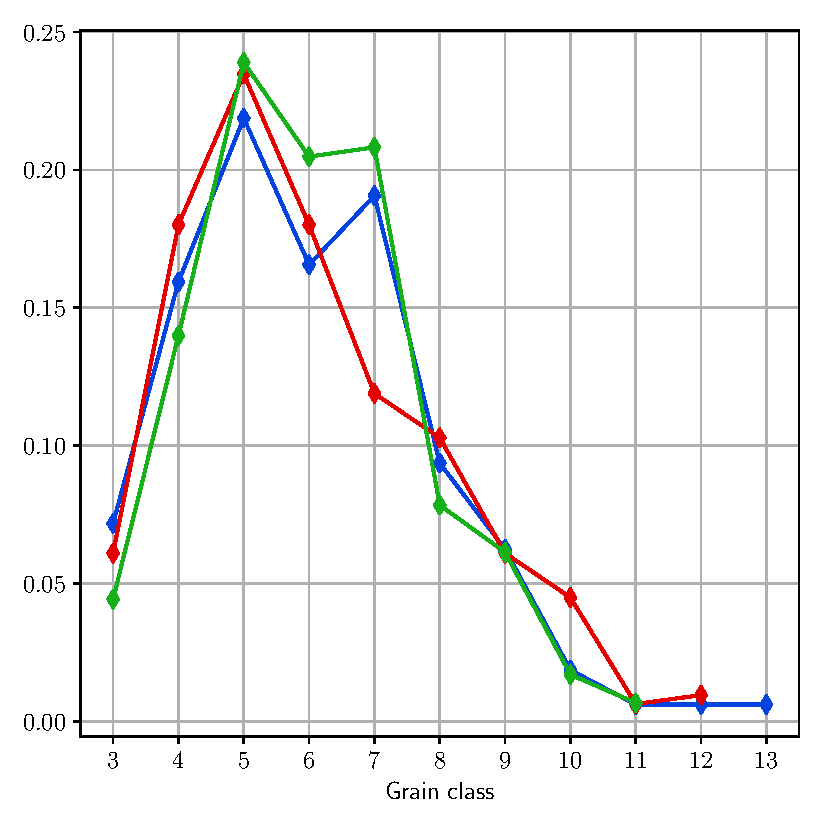
\includegraphics[scale=0.45, trim={0em 0 0em 0}]{figures/stored_energy/SE/nsides/000240_nuclconstant_set.pdf}
    \label{fig:SE_nsides_3}
    }%
\caption{Average number of sides distributions at different stages of grain network evolution and nucleation with $\alpha = 0$.}
    \label{fig:SE_nsides}
\end{figure}

Stored energy distribution is shown in Figure~\ref{fig:SE_se}. Figure~\ref{fig:SE_se_0} shows the initial condition distribution. 
In dark blue the triangular distribution from \eqref{eq:triangular_dist} is shown. After the first grain growth regime and first nucleations the distribution shows a clear tendency to remove grains with high values of stored energy and maintain those with lower values. Nucleated grains appear in the plot with stored energy equal to zero, as shown in Figure~\ref{fig:SE_se_1}. During the nucleation the grains with less stored energy still survives but will be removed no matter what happens, as shown in Figure~\ref{fig:SE_se_2}. Figure~\ref{fig:SE_se_3} shows the final stage of recrystallization where there are no grains with store energy.

\begin{figure}[ht]
    \centering
    \subfloat[Initial condition.]{
    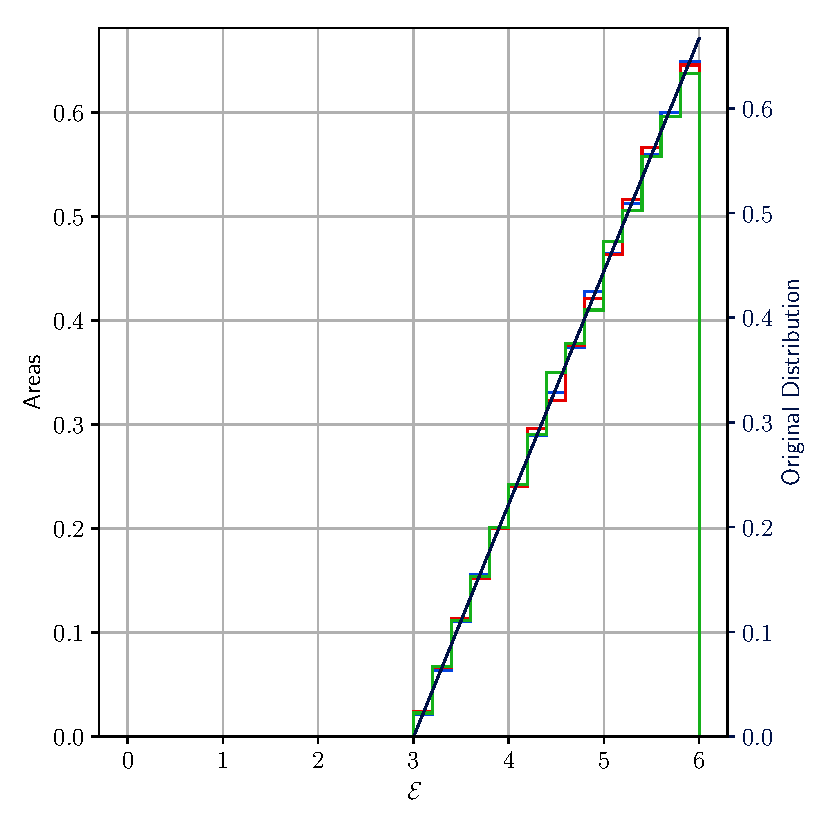
\includegraphics[scale=0.45, trim={0em 0 0em 0}]{figures/stored_energy/SE/se/000000_nuclconstant_set.pdf}
    \label{fig:SE_se_0}
    }%
    \subfloat[First nucleations.]{
    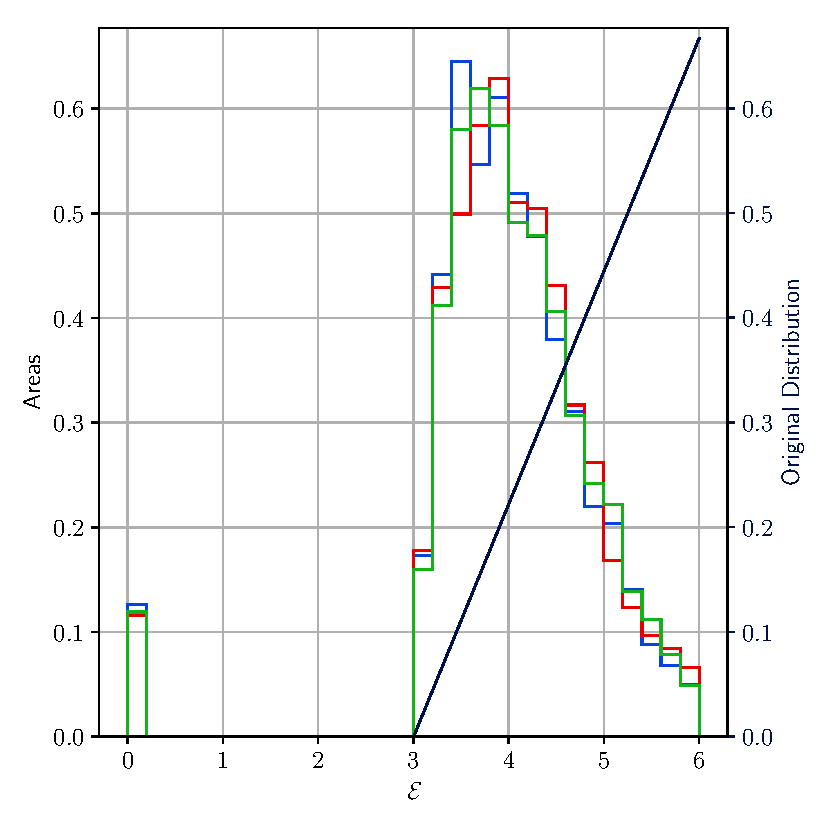
\includegraphics[scale=0.45, trim={0em 0 0em 0}]{figures/stored_energy/SE/se/000070_nuclconstant_set.pdf}
    \label{fig:SE_se_1}
    }\\%
    %\hspace{-4.5em}
    \subfloat[Nucleation stage.]{
    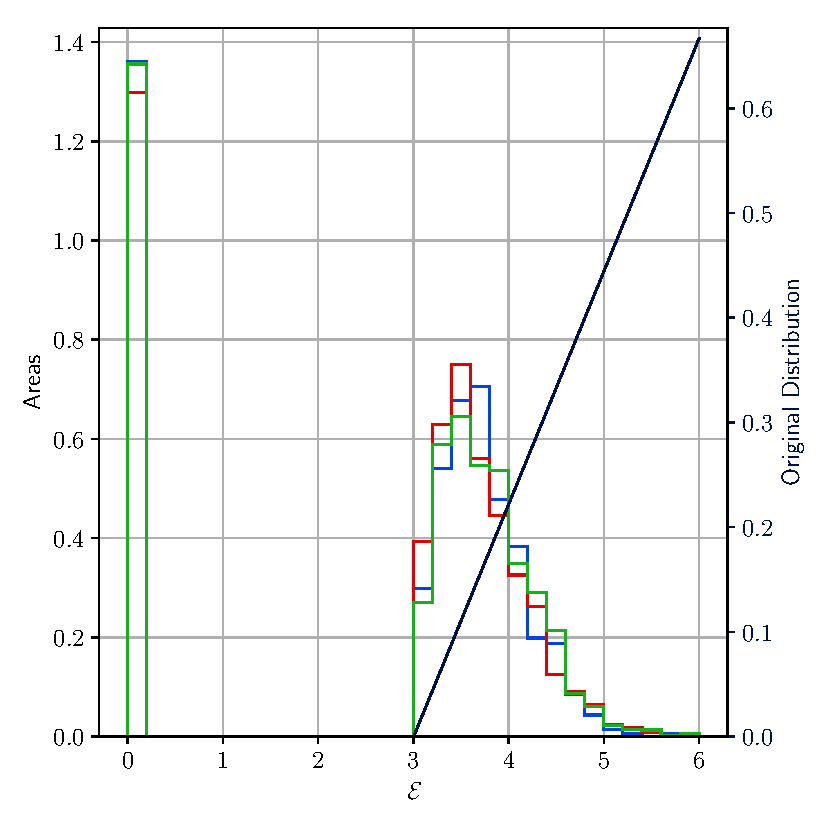
\includegraphics[scale=0.45, trim={0em 0 0em 0}]{figures/stored_energy/SE/se/000110_nuclconstant_set.pdf}
    \label{fig:SE_se_2}
    }%
    \subfloat[Recrystallization.]{
    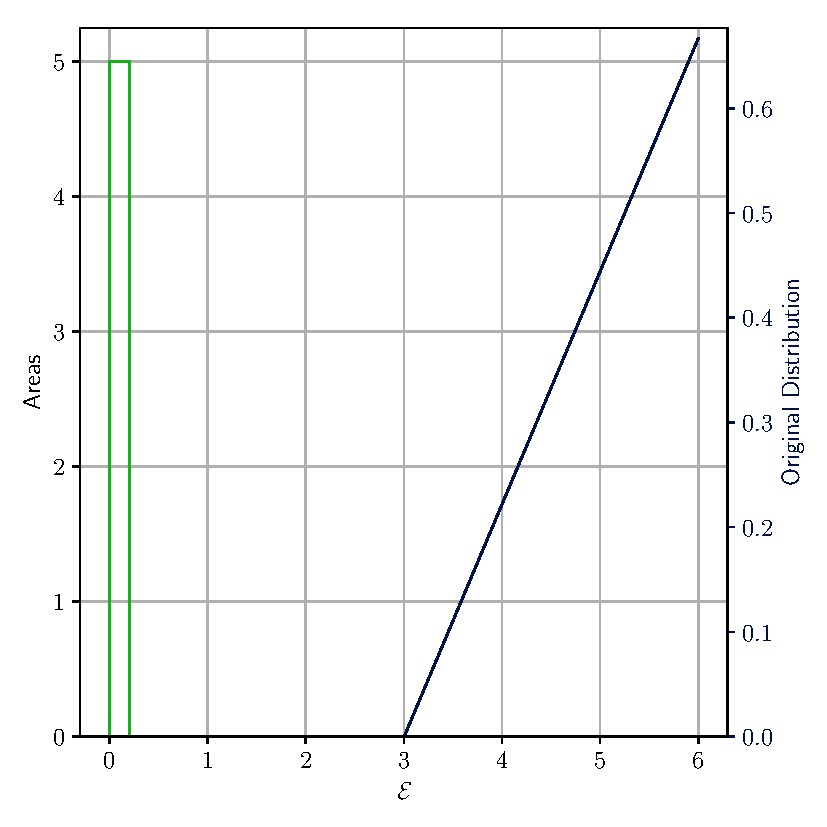
\includegraphics[scale=0.45, trim={0em 0 0em 0}]{figures/stored_energy/SE/se/000240_nuclconstant_set.pdf}
    \label{fig:SE_se_3}
    }%
\caption{Stored energy distributions at different stages of grain network evolution and nucleation with $\alpha = 0$.}
    \label{fig:SE_se}
\end{figure}

%%%%% Nucleation alternative %%%%%%%%%%%%%%

\subsection{Statistics for Model with Alternative Nucleation}

Similar to Section~\ref{sec:stats_basicnucl}, we present the evolution stages of the grain network in Figure~\ref{fig:SEnucl2_evolution}. Figure~\ref{fig:SEnucl2_dist_0} shows the same initial condition as Figure~\ref{fig:SE_dist_0}. Figure~\ref{fig:SEnucl2_dist_1} shows first nucleations in the grain network. 
Those grains are initialized with $\SE = 0$ and $\alpha = \alpha_{\text{nucl}}$ which was computed from \eqref{eq:minalpha}. As discussed in Section~\ref{sec:alternative_nucleation}, we generate $\alpha_{\text{nucl}}$ from a sampling over $[0,2\pi)$ using $500$ discretization points.

After some time the nucleated grains will start to increase its number of sides as seen in Figure~\ref{fig:SEnucl2_dist_2}. 
Finally, Figure~\ref{fig:SEnucl2_dist_3} shows a fully recrystallized grain network. We do not expect in the final recrystallization an isotropic grain network since in general $\Delta \alpha \neq 0$, that is, we do not enforce isotropy. 
However, we do use stored energy zero for nucleated grains, therefore this stage represents an anisotropic vertex model, which has the following energy equation:
\begin{equation*}
    E = \sum_{k=1}^{K} \gamma^{(k)}\AL_k.
\end{equation*}
%
\begin{figure}[ht]
    \centering
    %\hspace{-4.5em}
    \subfloat[Zoom of Initial distribution generated via Voronoi tessellation.]{
    \includegraphics[scale=0.40, trim={2em 0 2em 0}]{figures/stored_energy/SEnucl2/snaps/000000.pdf}
    \label{fig:SEnucl2_dist_0}
    }%
    \subfloat[First nucleations.]{
    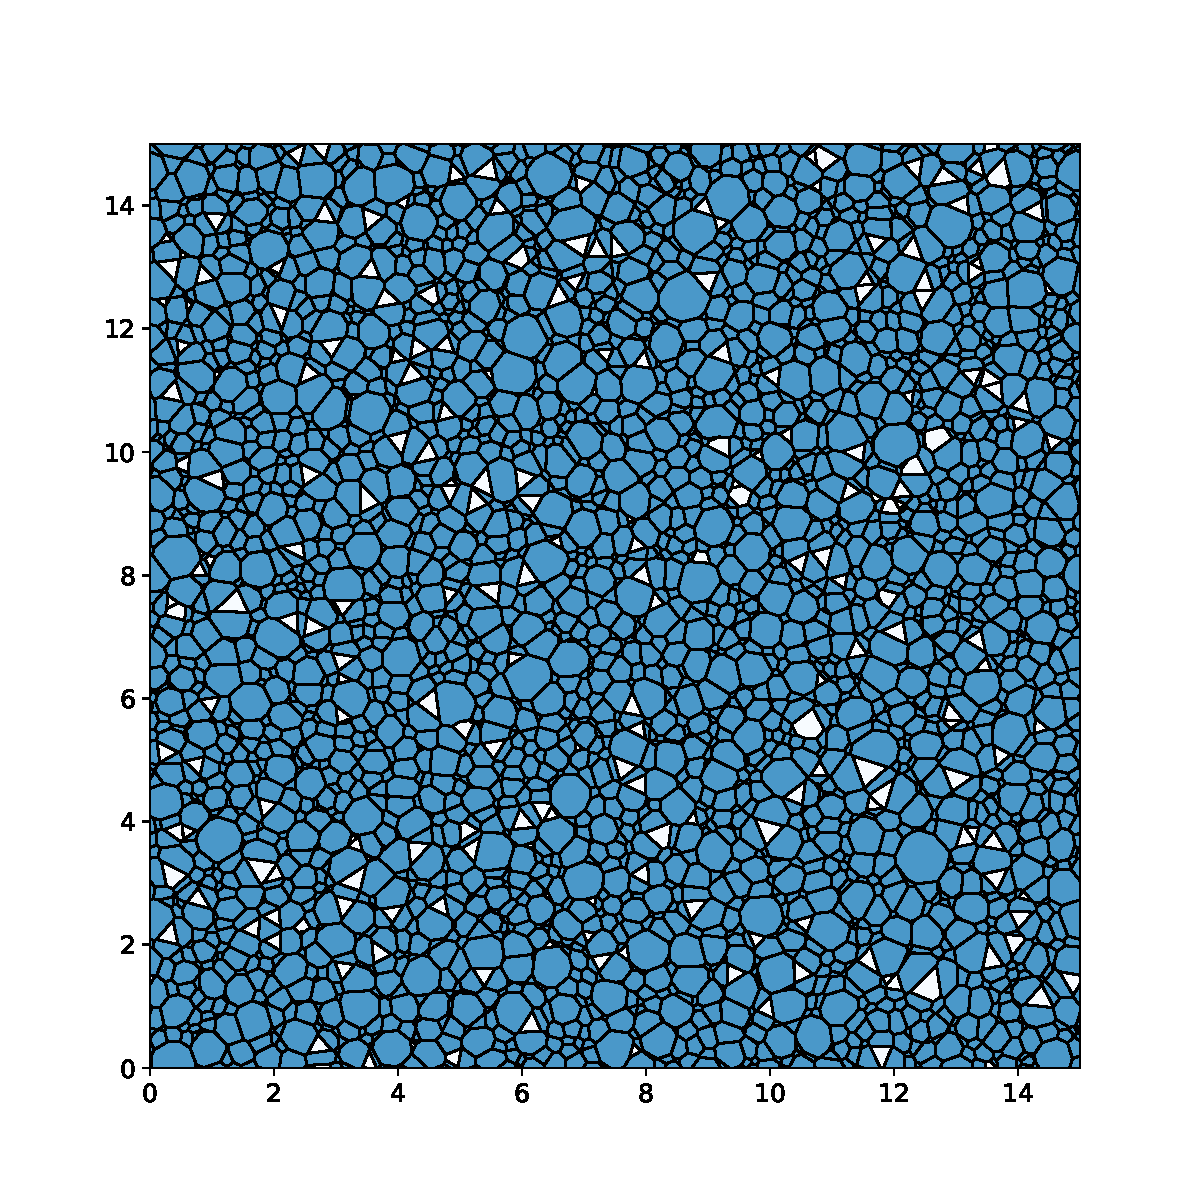
\includegraphics[scale=0.40, trim={2em 0 2em 0}]{figures/stored_energy/SEnucl2/snaps/000070.pdf}
    \label{fig:SEnucl2_dist_1}
    }\\%
    %\hspace{-4.5em}
    \subfloat[Nucleation stage.]{
    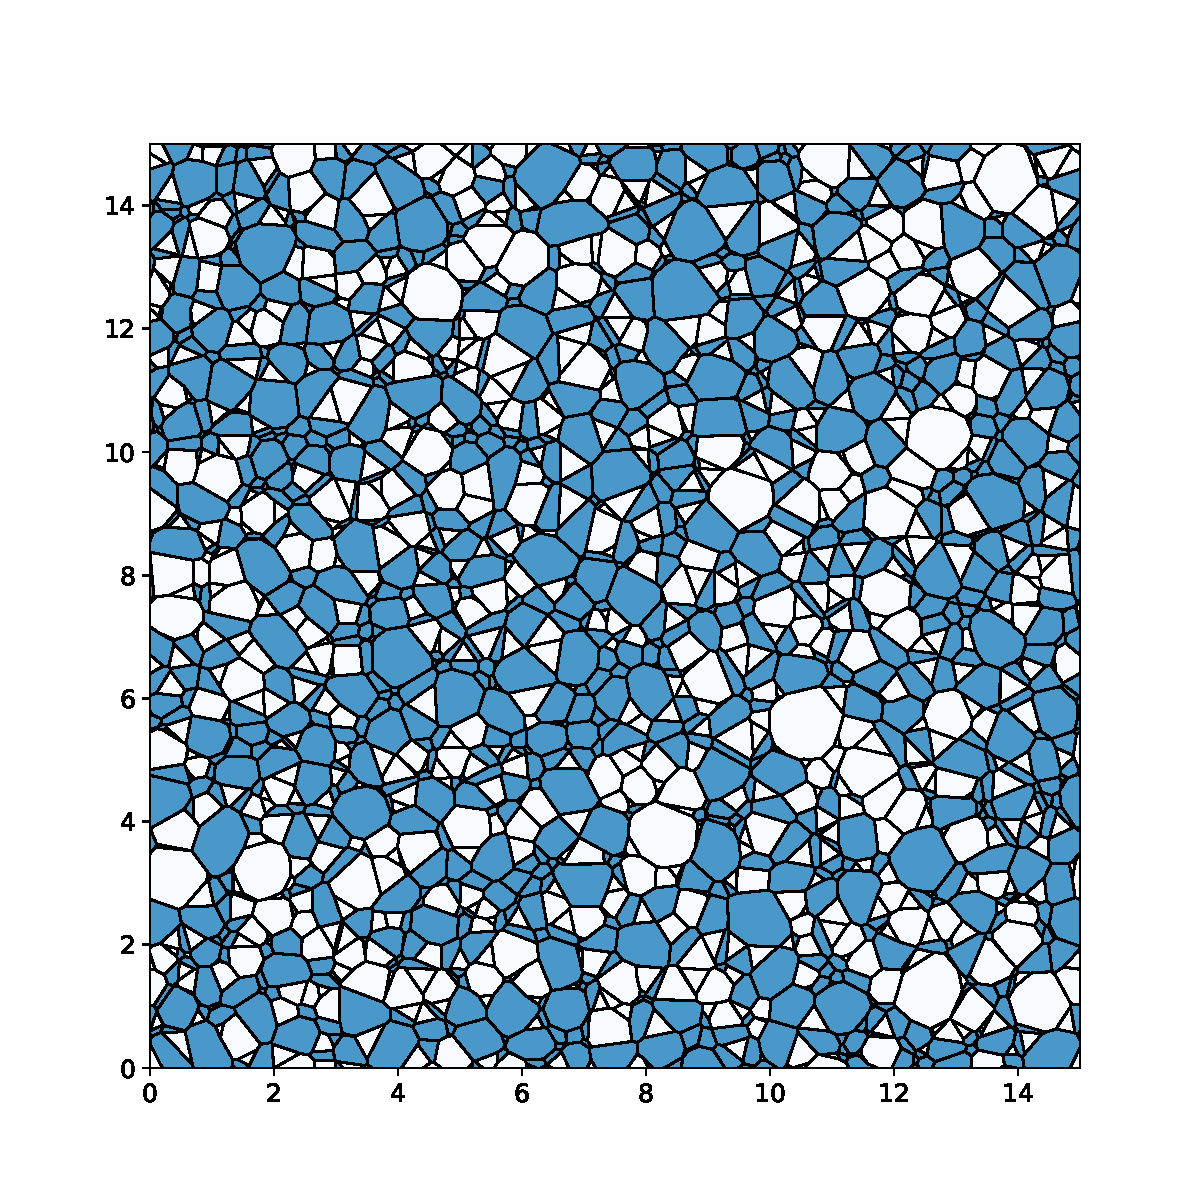
\includegraphics[scale=0.40, trim={2em 0 2em 0}]{figures/stored_energy/SEnucl2/snaps/000110.pdf}
    \label{fig:SEnucl2_dist_2}
    }%
    \subfloat[Recrystallization.]{
    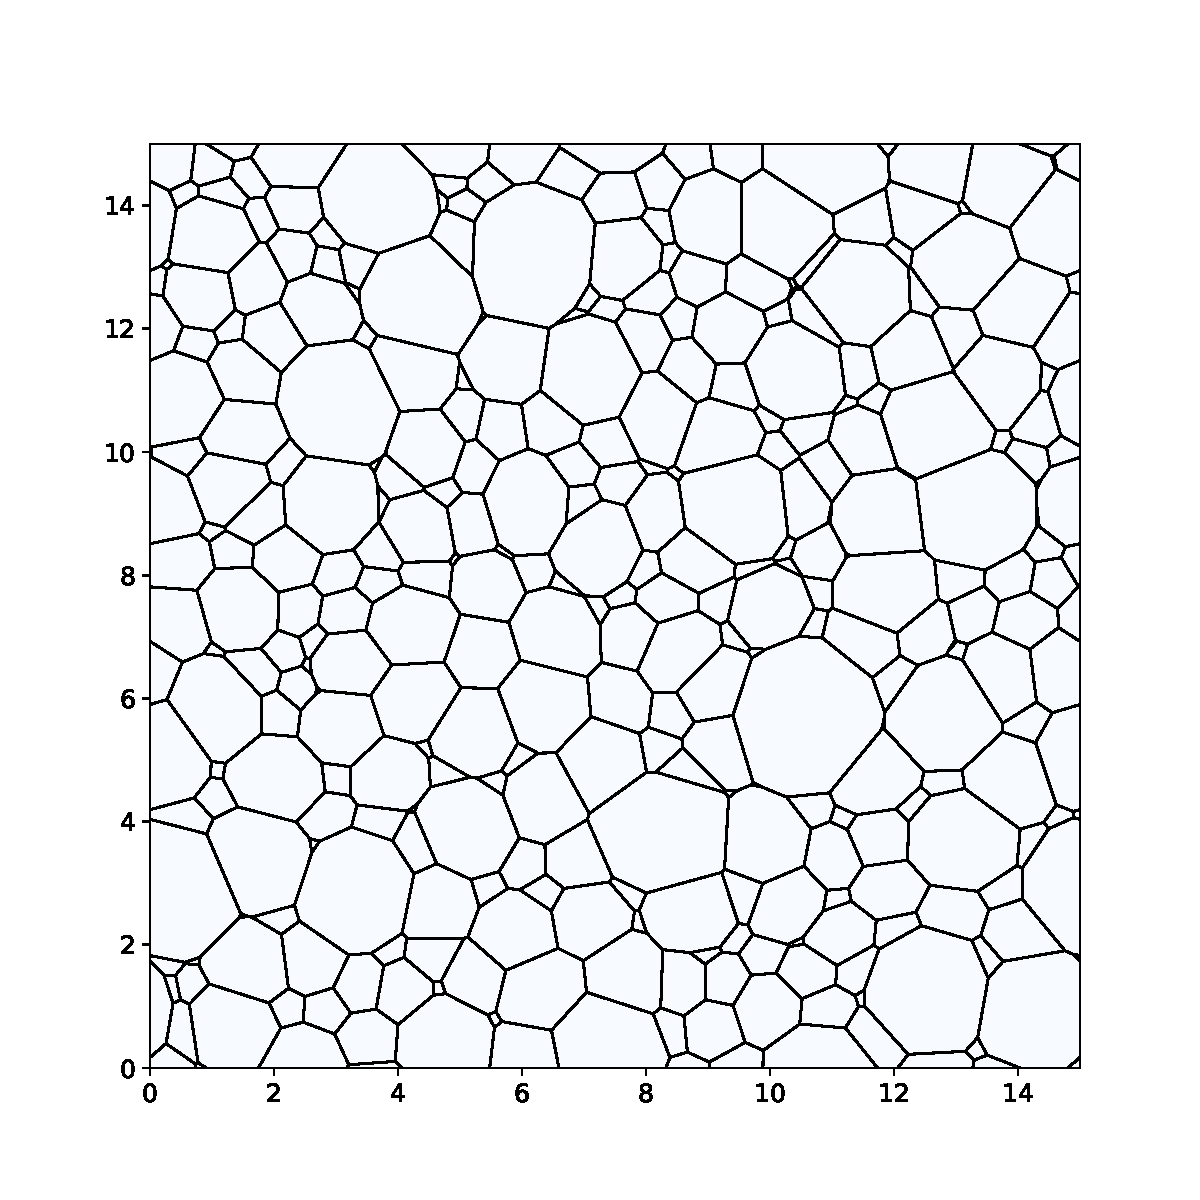
\includegraphics[scale=0.40, trim={2em 0 2em 0}]{figures/stored_energy/SEnucl2/snaps/000240.pdf}
    \label{fig:SEnucl2_dist_3}
    }%
    \caption{Stages of grain network evolution nucleating with $\alpha = \alpha_{\text{nucl}}$.}
    \label{fig:SEnucl2_evolution}
\end{figure}
%%% AREAS

Area distribution is shown in Figure~\ref{fig:SEnucl2_areas} in both linear and logarithmic scale.  Figure~\ref{fig:SEnucl2_areas_0} shows the initial condition distribution. Figure~\ref{fig:SEnucl2_areas_1} shows the distribution during the first nucleations, which again resembles the Vertex model area distribution. Figures~\ref{fig:SEnucl2_areas_2} and~\ref{fig:SEnucl2_areas_3} shows that the distributions over time are similar.

\begin{figure}[ht]
    \vspace{-1em}
    \centering
    \subfloat[Initial condition.]{
    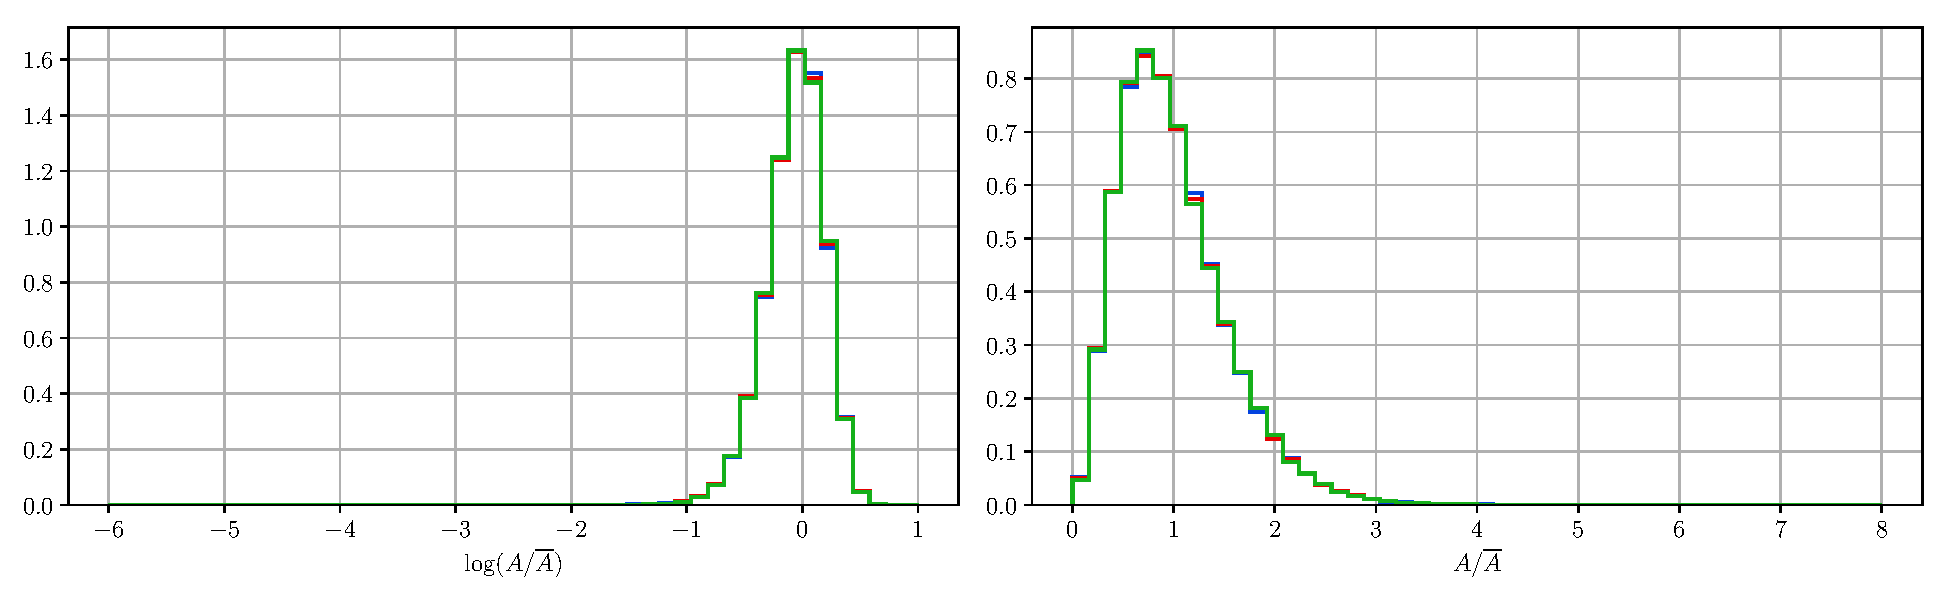
\includegraphics[scale=0.42, trim={0em 1em 0em 2em}]{figures/stored_energy/SE/areas/000000_nuclalternative_set.pdf}
    \label{fig:SEnucl2_areas_0}
    }\\
    \subfloat[First nucleations.]{
    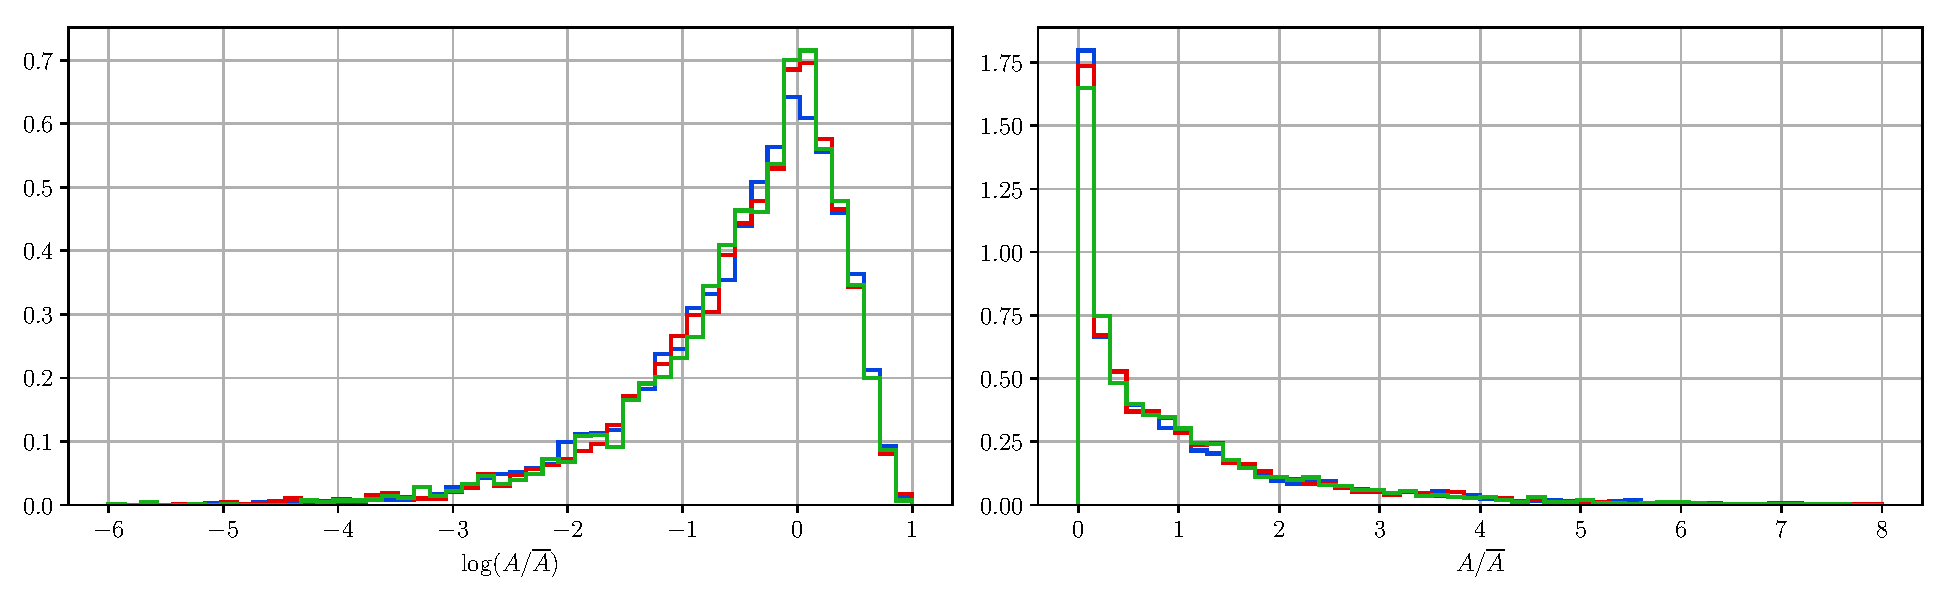
\includegraphics[scale=0.42, trim={0em 1em 0em 2em}]{figures/stored_energy/SE/areas/000070_nuclalternative_set.pdf}
    \label{fig:SEnucl2_areas_1}
    }\\%
    %\hspace{-4.5em}
    \subfloat[Nucleation stage.]{
    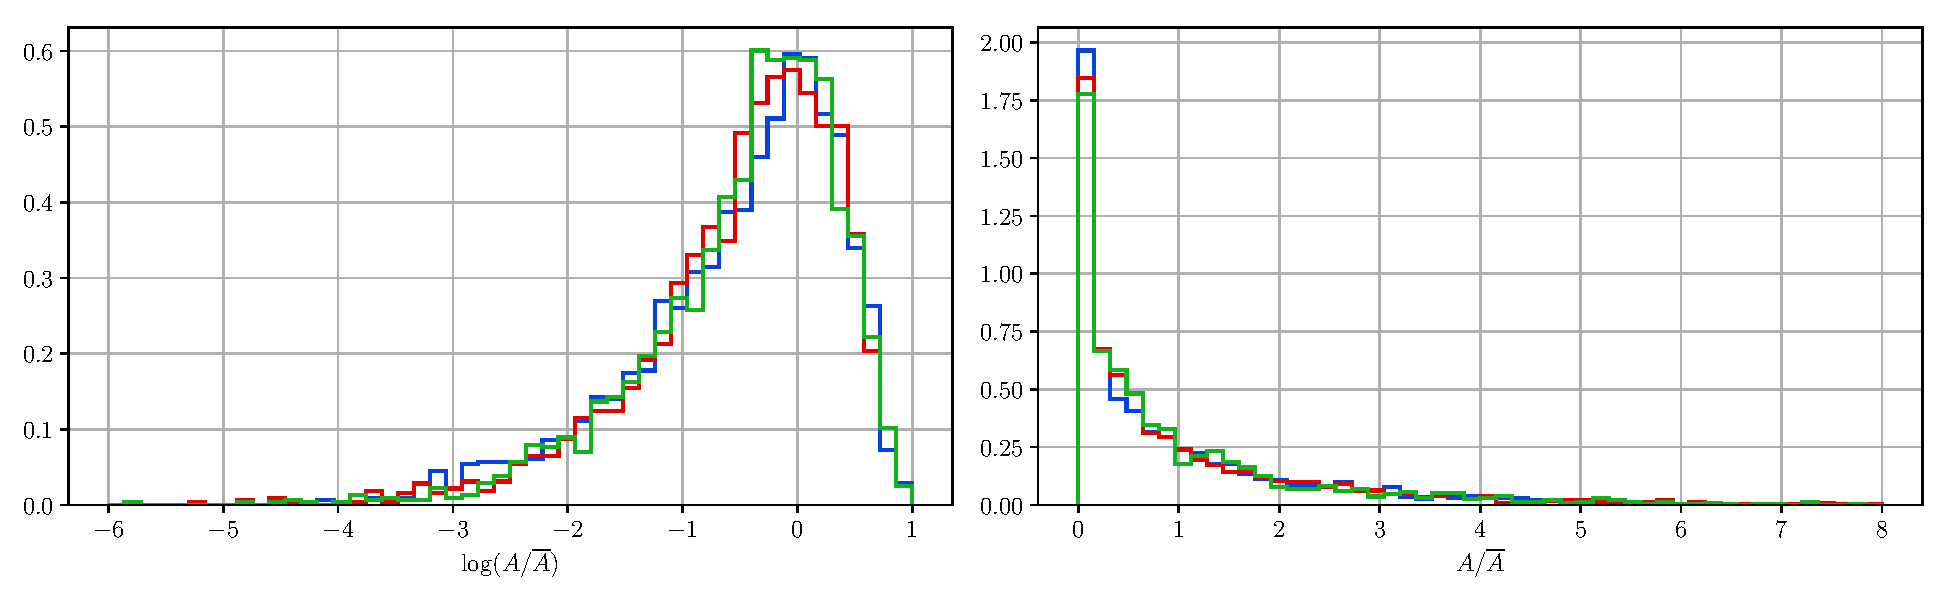
\includegraphics[scale=0.42, trim={0em 1em 0em 2em}]{figures/stored_energy/SE/areas/000110_nuclalternative_set.pdf}
    \label{fig:SEnucl2_areas_2}
    }\\%
    \subfloat[Recrystallization.]{
    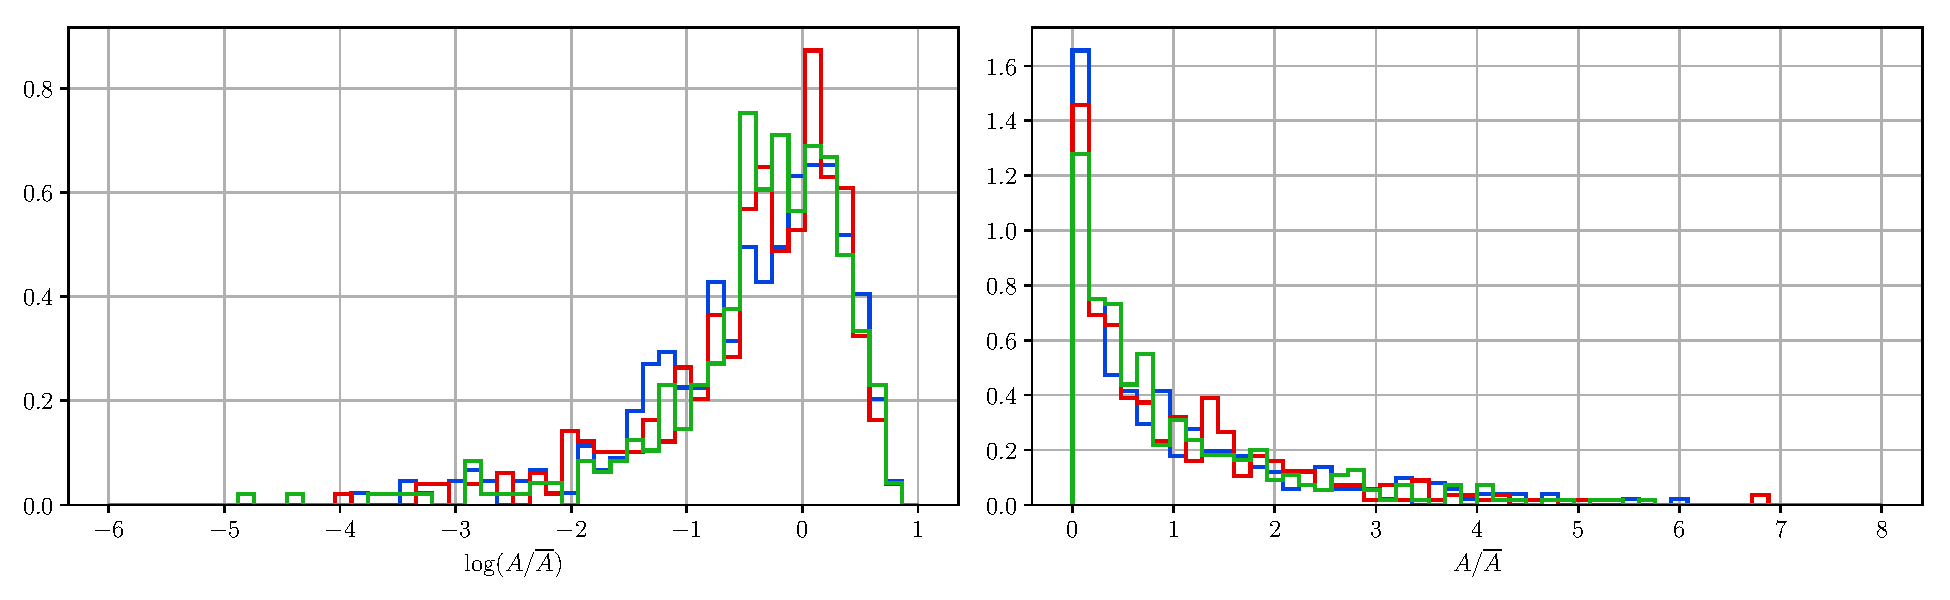
\includegraphics[scale=0.42, trim={0em 1em 0em 2em}]{figures/stored_energy/SE/areas/000240_nuclalternative_set.pdf}
    \label{fig:SEnucl2_areas_3}
    }%
    \caption{Grain relative area distributions at different stages of grain network evolution and nucleation with $\alpha = \alpha_{\text{nucl}}$.}
    \label{fig:SEnucl2_areas}
\end{figure}
%
Figure~\ref{fig:SEnucl2_dihedral} shows the dihedral angle distribution.
The distributions shown at different stages of the growth are similar to those from Figure~\ref{fig:SE_dihedral}, showing the same bimodal behavior related to the thin and large grains being removed during the nucleation stage in Figure~\ref{fig:SEnucl2_dihedral_2} with the particularity that the bimodal seems to be more pronounced in earlier steps as seen in Figure~\ref{fig:SEnucl2_dihedral_1}. The distribution again stabilizes when the structure is fully recrystallizated in Figure~\ref{fig:SEnucl2_dihedral_3}.

\begin{figure}[ht]
    \centering
    \subfloat[Initial condition.]{
    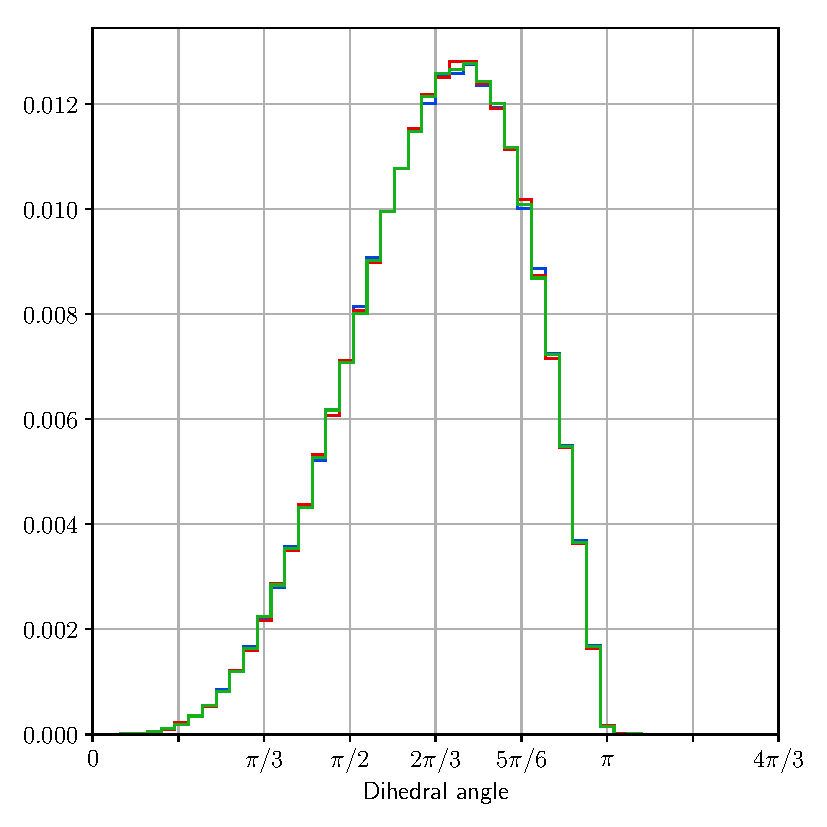
\includegraphics[scale=0.43, trim={0em 0 0em 0}]{figures/stored_energy/SE/dihedral/000000_nuclalternative_set.pdf}
    \label{fig:SEnucl2_dihedral_0}
    }%
    \subfloat[First nucleations.]{
    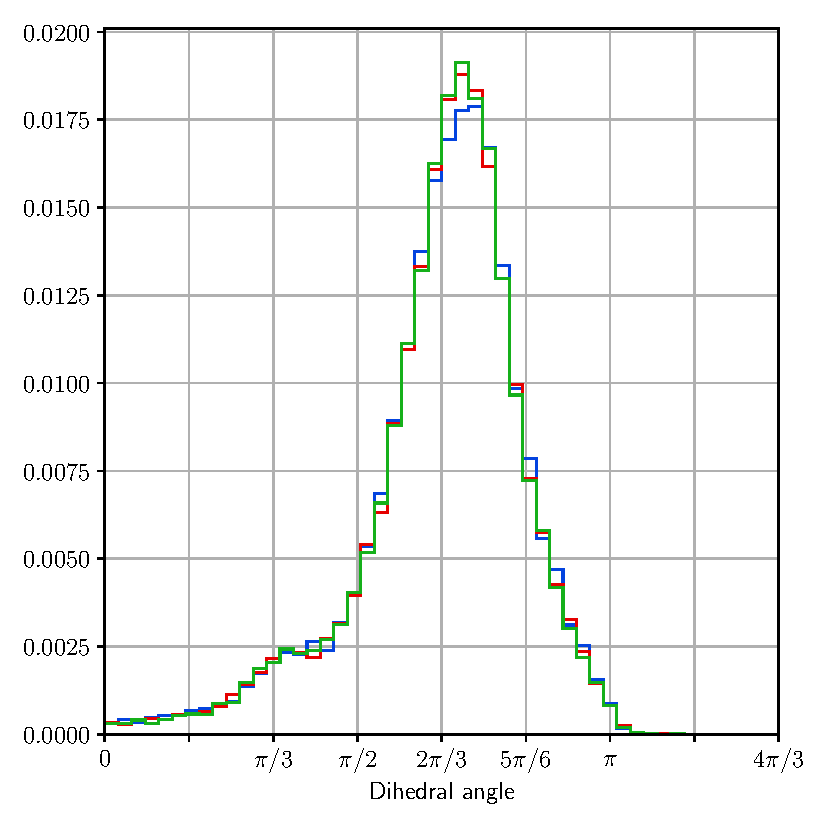
\includegraphics[scale=0.43, trim={0em 0 0em 0}]{figures/stored_energy/SE/dihedral/000070_nuclalternative_set.pdf}
    \label{fig:SEnucl2_dihedral_1}
    }\\%
    %\hspace{-4.5em}
    \subfloat[Nucleation stage.]{
    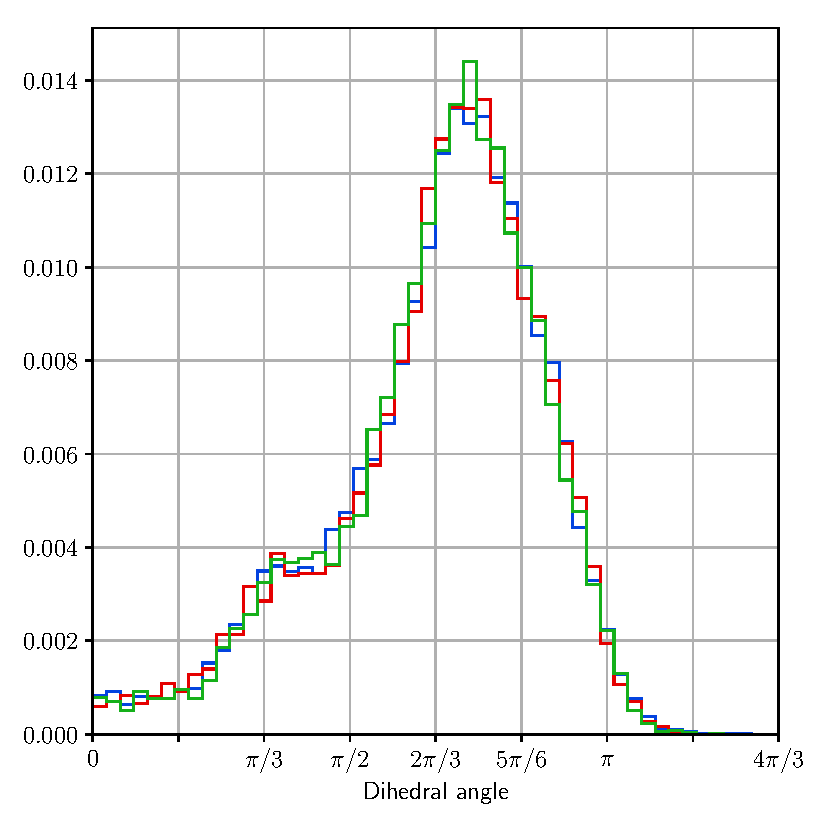
\includegraphics[scale=0.43, trim={0em 0 0em 0}]{figures/stored_energy/SE/dihedral/000110_nuclalternative_set.pdf}
    \label{fig:SEnucl2_dihedral_2}
    }%
    \subfloat[Recrystallization.]{
    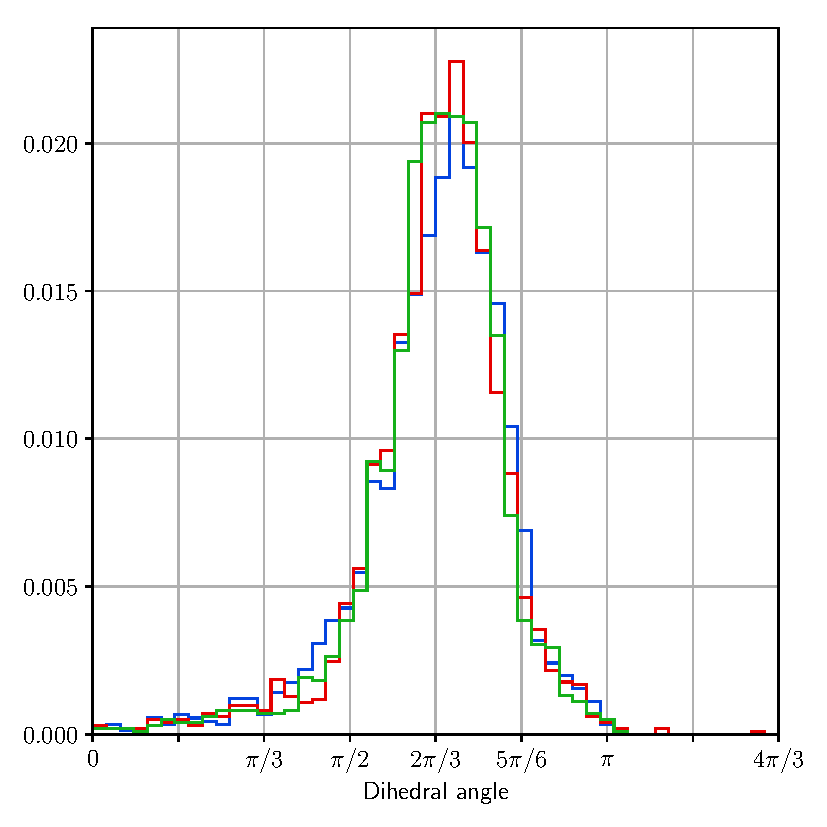
\includegraphics[scale=0.43, trim={0em 0 0em 0}]{figures/stored_energy/SE/dihedral/000240_nuclalternative_set.pdf}
    \label{fig:SEnucl2_dihedral_3}
    }%
\caption{Dihedral angle distributions at different stages of grain network evolution and nucleation with $\alpha = \alpha_{\text{nucl}}$.}
    \label{fig:SEnucl2_dihedral}
\end{figure}


Grain boundary character distribution (GBCD) is shown in Figure~\ref{fig:SEnucl2_gbcd}. 
Dark blue line shows the grain boundary energy function from \eqref{eq:gamma}. 
The initial uniform GBCD is shown in Figure~\ref{fig:SEnucl2_gbcd_0}. Figure~\ref{fig:SEnucl2_gbcd_1} shows the GBCD just after grain growth and first nucleations.
There are more steep slopes, related to the inflection angles $-\pi/4, 0$ and $\pi/4$ and also due to the misorientation choice for nucleated grains which is no longer zero but an approximation to a local energy minimizer which helps to preserve the distribution. Figure~\ref{fig:SEnucl2_gbcd_2} shows the GBCD at the nucleation stage, which clearly has minimum at misorientation angles $\pm \pi/4$ and maximum at $0$. 
Notice the local maximum reached near $\pm \pi/8$ and where the energy function has its inflection points.
%also has derivative zero in this interval. 
%In fact this is the same behavior of the second derivative of \eqref{eq:gamma}.
Figure~\ref{fig:SEnucl2_gbcd_3} shows the GBCD after full recrystallization. 
Since the recrystallized structure holds different values of orientations, this regime is anisotropic and thus the GBCD is not uniform and preserves some behavior of early stages.


\begin{figure}[ht]
    \centering
    \subfloat[Initial condition.]{
    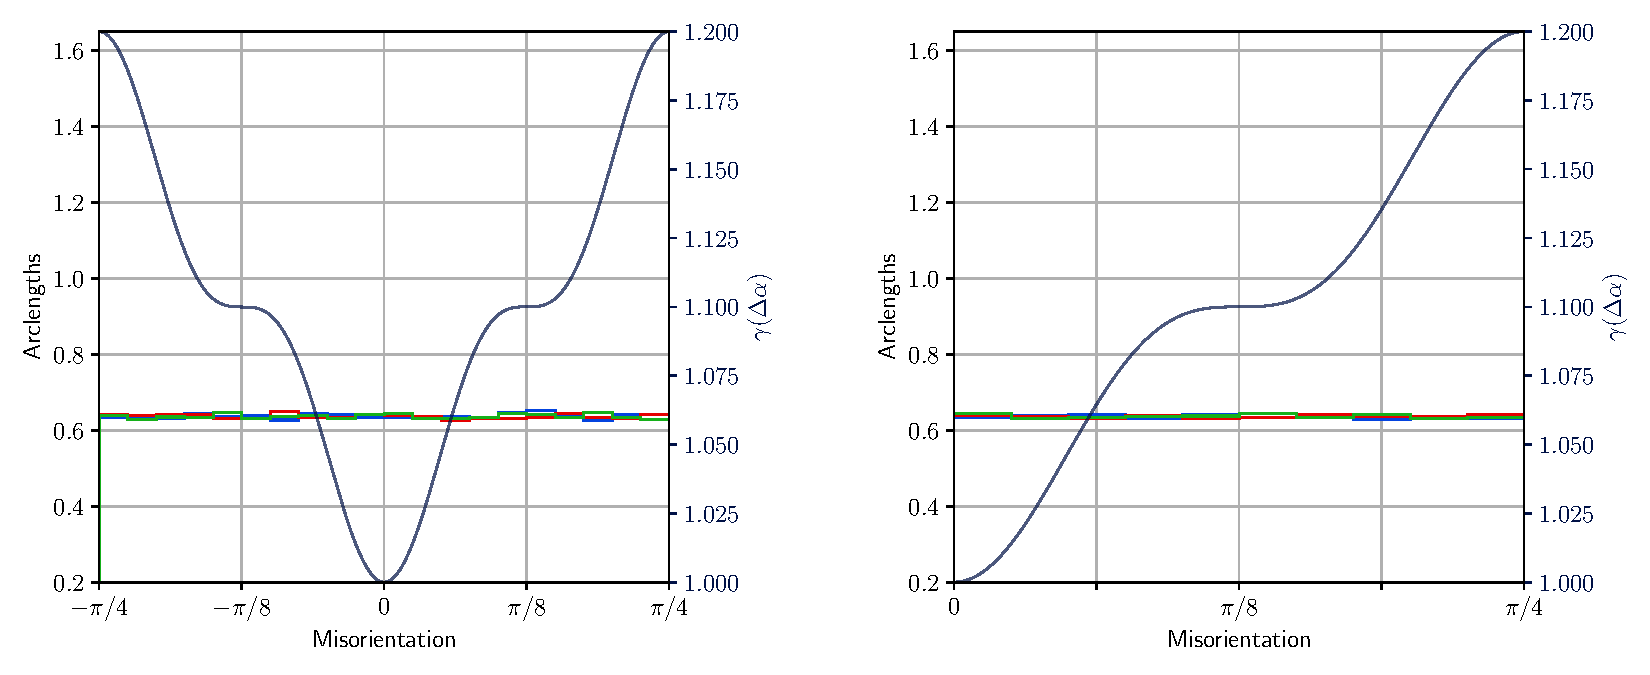
\includegraphics[scale=0.5, trim={0em 0 0em 0}]{figures/stored_energy/SE/gbcd/000000_nuclalternative_set.pdf}
    \label{fig:SEnucl2_gbcd_0}
    }\\
    \subfloat[First nucleations.]{
    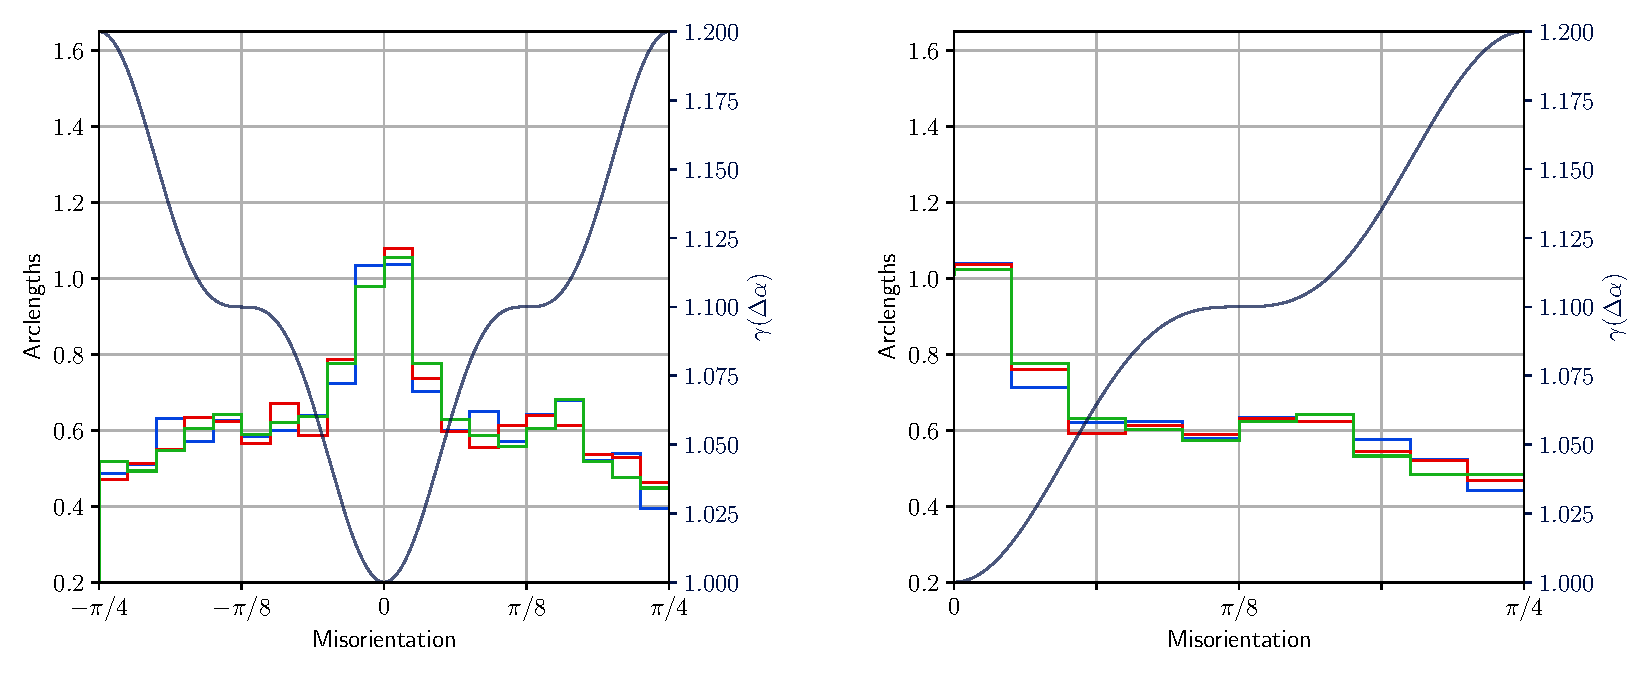
\includegraphics[scale=0.5, trim={0em 0 0em 0}]{figures/stored_energy/SE/gbcd/000070_nuclalternative_set.pdf}
    \label{fig:SEnucl2_gbcd_1}
    }
    \caption{Grain Boundary Character distributions at different stages of grain network evolution and nucleation with $\alpha = \alpha_{\text{nucl}}$.}
\end{figure}
\begin{figure}[ht]\ContinuedFloat
    \centering
    \subfloat[Nucleation stage.]{
    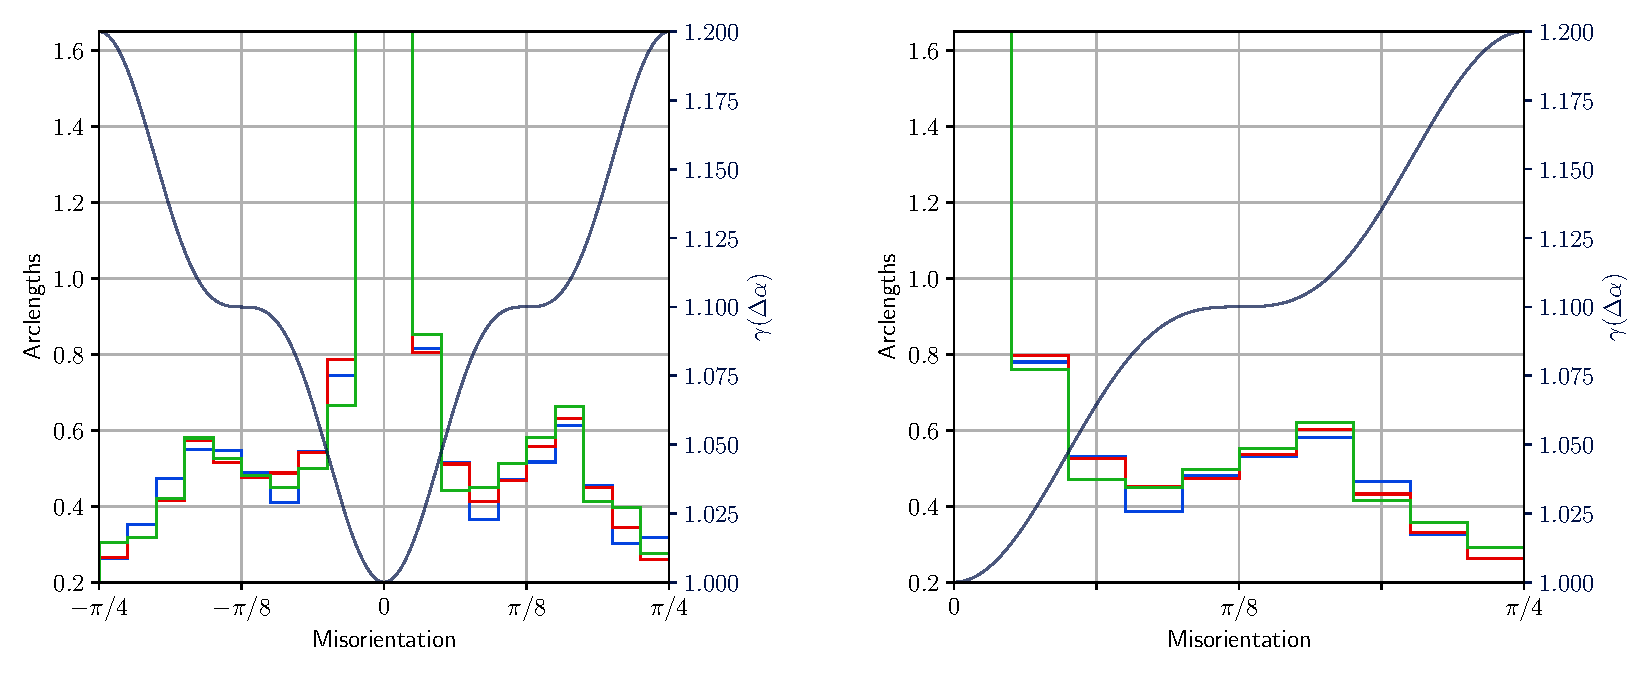
\includegraphics[scale=0.5, trim={0em 0 0em 0}]{figures/stored_energy/SE/gbcd/000110_nuclalternative_set.pdf}
    \label{fig:SEnucl2_gbcd_2}
    }\\
    \subfloat[Recrystallization.]{
    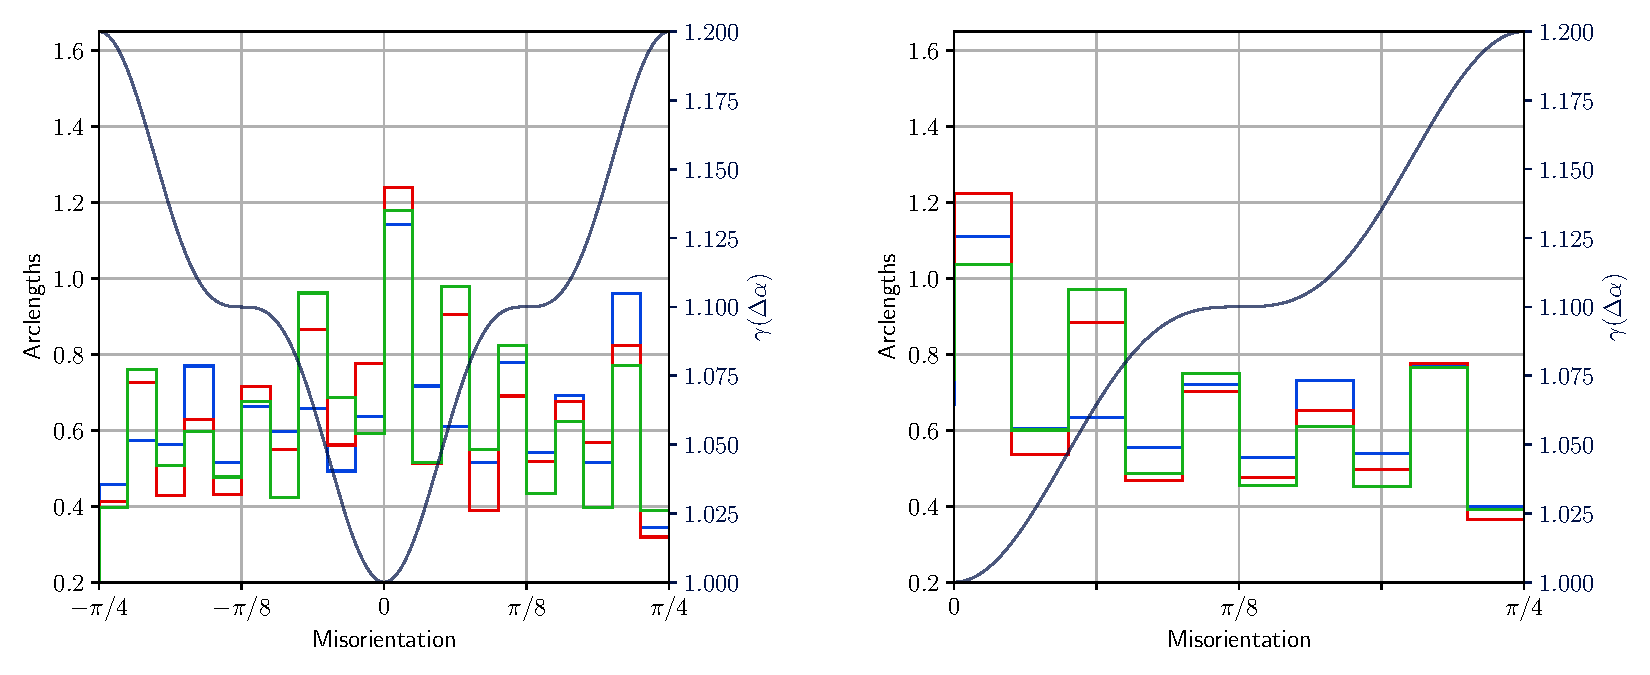
\includegraphics[scale=0.5, trim={0em 0 0em 0}]{figures/stored_energy/SE/gbcd/000240_nuclalternative_set.pdf}
    \label{fig:SEnucl2_gbcd_3}
    }
    \caption{Grain Boundary Character distributions at different stages of grain network evolution and nucleation with $\alpha = \alpha_{\text{nucl}}$. (Cont.)}
    \label{fig:SEnucl2_gbcd}
\end{figure}

Distribution of average number of sides is shown in Figure~\ref{fig:SEnucl2_nsides}. 
The behavior is very similar comparing to the nucleation model with $\alpha = 0$ in Figure~\ref{fig:SE_nsides} where the four plots reflects the growth stage and first nucleations in Figure~\ref{fig:SEnucl2_nsides_1}, nucleation stage in Figure~\ref{fig:SEnucl2_nsides_2} and recrystallization stage in Figure~\ref{fig:SEnucl2_nsides_3} where the mode of the average number of sides is five. In general the distributions are more regular than the other nucleation model and preserve the same characteristics.

\begin{figure}[ht]
    \centering
    \subfloat[Initial condition.]{
    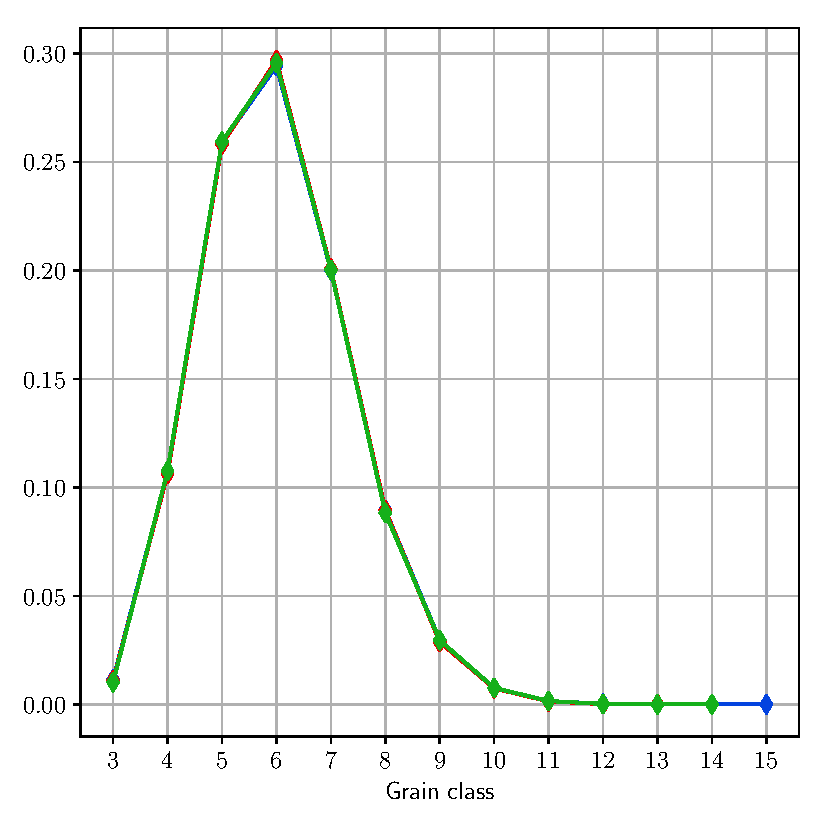
\includegraphics[scale=0.5, trim={0em 0 0em 0}]{figures/stored_energy/SE/nsides/000000_nuclalternative_set.pdf}
    \label{fig:SEnucl2_nsides_0}
    }%
    \subfloat[First nucleations.]{
    \includegraphics[scale=0.5, trim={0em 0 0em 0}]{figures/stored_energy/SE/nsides/000070_nuclalternative_set.pdf}
    \label{fig:SEnucl2_nsides_1}
    }\\%
    %\hspace{-4.5em}
    \subfloat[Nucleation stage.]{
    \includegraphics[scale=0.5, trim={0em 0 0em 0}]{figures/stored_energy/SE/nsides/000110_nuclalternative_set.pdf}
    \label{fig:SEnucl2_nsides_2}
    }%
    \subfloat[Recrystallization.]{
    \includegraphics[scale=0.5, trim={0em 0 0em 0}]{figures/stored_energy/SE/nsides/000240_nuclalternative_set.pdf}
    \label{fig:SEnucl2_nsides_3}
    }%
    \caption{Average number of sides distributions at different stages of grain network evolution and nucleation with $\alpha = \alpha_{\text{nucl}}$.}
    \label{fig:SEnucl2_nsides}
\end{figure}

Stored energy distribution is shown in Figure~\ref{fig:SEnucl2_se}.
Figure~\ref{fig:SEnucl2_se_0} shows the initial condition distribution. 
In dark blue the triangular distribution from \eqref{eq:triangular_dist} is shown. Similar to the nucleation model with $\alpha = 0$, we observe in Figure~\ref{fig:SEnucl2_se_1} that after initial growth and first nucleations, the distribution tends to preserve grains with lower stored energy values as well as showing a bin at zero stored energy related to nucleated grains.
Figure~\ref{fig:SEnucl2_se_2} shows that during the nucleation stage the tendency of the energy minimization via removing grains with high stored energy values is maintained and finally in Figure~\ref{fig:SEnucl2_se_3} the only residual bin of the distribution is at zero which marks the existence of the fully recrystallization structure where the stored energy does not influences the system anymore.

\begin{figure}[ht]
    \centering
    \subfloat[Initial condition.]{
    \includegraphics[scale=0.45, trim={0em 0 0em 0}]{figures/stored_energy/SE/se/000000_nuclalternative_set.pdf}
    \label{fig:SEnucl2_se_0}
    }%
    \subfloat[First nucleations.]{
    \includegraphics[scale=0.45, trim={0em 0 0em 0}]{figures/stored_energy/SE/se/000070_nuclalternative_set.pdf}
    \label{fig:SEnucl2_se_1}
    }\\%
    %\hspace{-4.5em}
    \subfloat[Nucleation stage.]{
    \includegraphics[scale=0.45, trim={0em 0 0em 0}]{figures/stored_energy/SE/se/000110_nuclalternative_set.pdf}
    \label{fig:SEnucl2_se_2}
    }%
    \subfloat[Recrystallization.]{
    \includegraphics[scale=0.45, trim={0em 0 0em 0}]{figures/stored_energy/SE/se/000240_nuclalternative_set.pdf}
    \label{fig:SEnucl2_se_3}
    }%
\caption{Stored energy distributions at different stages of grain network evolution and nucleation with $\alpha = \alpha_{\text{nucl}}$.}
    \label{fig:SEnucl2_se}
\end{figure}